\documentclass[a4paper,11pt,twoside,openright]{report}

\usepackage{graphicx}
%\usepackage{ngerman}
\usepackage[utf8x]{inputenc}
\usepackage{fancyvrb}
\usepackage{courier}
\usepackage{helvet}
\usepackage{tikz}
\usepackage{xcolor}
\usepackage{pdfpages}
\usetikzlibrary{calc}
\usepackage[strict]{changepage}
\usepackage{xspace}
\usepackage{hyperref}
\usepackage{cleveref}
\usetikzlibrary{shapes.geometric}
\usetikzlibrary{arrows}
\usetikzlibrary{positioning}
\usetikzlibrary{arrows.meta, automata, shapes, matrix,positioning}
\usepackage{amssymb}
\usepackage{pifont}% http://ctan.org/pkg/pifont
\usepackage{amsmath}
\usepackage{subcaption} 
\usepackage{float}
\usepackage{fixfoot}
\usepackage{graphicx}
\usepackage{wrapfig}

\pdfoptionpdfminorversion=6

% \definecolor{se_dark_blue}{RGB}{0,103,166} % powerpoint
\definecolor{se_dark_blue}{RGB}{0,96,178} % website
% \definecolor{se_light_blue}{RGB}{119,158,201} % powerpoint
\definecolor{se_light_blue}{RGB}{129,160,225} % website


%% setup listings
\usepackage{listings}
\lstset{
    numberstyle=\tiny,
    numbersep=5pt,
    xleftmargin=11pt,
    xrightmargin=4pt,
    aboveskip=0pt,
    belowskip=-6pt,
    sensitive=true,
    float=!t,
    breaklines=false,
    captionpos=b,
    tabsize=2,
    showstringspaces=false,
    basicstyle=\small\ttfamily,
    morecomment=[l]{//},
    morecomment=[s][\itshape]{/**}{*/}
}

%% defines the listings laguage named 'MontiArc' derived from the language 'Java' 
%% adding the below listed keywords. See 
%% ftp://ftp.tex.ac.uk/tex-archive/macros/latex/contrib/listings/listings.pdf
%% for listings documentation
\lstdefinelanguage{MontiArc}[]{Java}{
  morekeywords={component, port, in, out, inv, package, import, connect, autoconnect}
}

% Seite einrichten
\setlength{\voffset}{-1in}
\setlength{\hoffset}{-1in}

\setlength{\topmargin}{2.5cm}		   
\setlength{\headheight}{0cm}		   
\setlength{\headsep}{0cm}		   
\setlength{\oddsidemargin}{3,3cm}  % innen ein wenig mehr Rand für die Klebebindung
\setlength{\evensidemargin}{2,7cm} % dafür außen ein wenig weniger
\setlength{\textwidth}{15cm}		   
\setlength{\textheight}{23,5cm}		   
\setlength{\parindent}{0cm}

% own commands
\newcommand{\red}[1]{\color{red}#1\color{black}}
\newcommand{\todoLine}{\noindent\rule{15cm}{0.4pt}}
\newcommand{\todo}[1]{\todoLine\\\red{TODO:}\xspace #1 \todoLine}
\newcommand{\cmark}{\ding{51}}%
\newcommand{\xmark}{\ding{55}}%

% Words
\newcommand{\emptyLine}{{\LARGE ~\\}}
\newcommand{\MontiCar}{MontiCar\xspace}
\newcommand{\kitti}{KITTI\xspace}
\newcommand{\cnnarch}{CNNArchLang\xspace}
\newcommand{\caffe}{Caffe\xspace}
\newcommand{\caffetwo}{Caffe2\xspace}
\newcommand{\mxnet}{MxNet\xspace}
\newcommand{\tensorflow}{Tensorflow\xspace}
\newcommand{\alexnet}{AlexNet\xspace}
\newcommand{\nn}{neural network\xspace}
\newcommand{\nns}{neural networks\xspace}
\newcommand{\torcs}{TORCS\xspace}
\newcommand{\alvinn}{ALVINN\xspace}

\DeclareFixedFootnote{\repnote}{ This is a repated footnote} 

\begin{document}

% Einrücken von Absätzen verhindern und 1.5 Zeilen Absatzabstand
\setlength{\parindent}{0pt}
\setlength{\parskip}{1.5ex plus0.5ex minus0.5ex}

%% Dieses Teildokument beschreibt die Titelseite.
%

% Seitenzähler auf 1, Römische Ziffern.
\setcounter{page}{1}
\pagenumbering{roman}

\thispagestyle{headings}

%\changepage{<text height>}{<text width>}{<even-side margin>}{<odd-side margin>}{<column sep.>}{<topmargin>}{<headheight>}{<headsep>}{<footskip>}
\changepage{5,1cm}{2.4cm}{}{-0.7cm}{}{-2,3cm}{}{}{}

% Eigentliche Titelseite.
\begin{titlepage}
	
\begin{figure}\raggedleft
\includegraphics[height=3.0cm]{src/pic/logo.jpg}\end{figure}
  
\begin{tikzpicture}[overlay]

% horizontal lines
\draw[color=se_dark_blue, thick] (-1.6, 0.9) -- (17.4, 0.9);
\draw[color=se_light_blue, thick] (-1.4, 0.7) -- (17.4, 0.7);

% vertical lines
\draw[color=se_dark_blue, thick] (-1, 0.9) -- (-1, -24.5);
\draw[color=se_light_blue, thick] (-0.8, 0.7) -- (-0.8, -24.5);

\end{tikzpicture}

\vspace*{-1.5em}

\begin{flushleft}
  {\fontfamily{phv}  
  	{\LARGE
      Rheinisch Westfälische Technische Hochschule Aachen \\
      Lehrstuhl für Software Engineering \\}
    \vspace{3em}
  
    {\LARGE \textbf{Erste Titel-Zeile}\\} 
    {\LARGE \textbf{Zweite Titel-Zeile}\\} 
    {\LARGE \textbf{Dritte Titel-Zeile}\\} % Oder \emptyLine falls nicht Titel kürzer
    {\LARGE \textbf{Vierte Titel-Zeile}\\} % Oder \emptyLine falls nicht Titel kürzer
    \vspace{3em}
		
    {\Large \textbf{Diplomarbeit/Masterarbeit/Studienarbeit}\\}
		\vspace{3em} 
		
		{\large von\\} % presented by
    
    {\LARGE \textbf{Name, Vorname}\\}
    \vspace{3em} 
		    
    {\Large \textbf{1. Prüfer: Prof.\ Dr.\ B.\ Rumpe}\\}
    \vspace{1em} 
    {\Large \textbf{2. Prüfer: }\\}
    \vspace{1em} 
    {\Large \textbf{Betreuer: }\\}
    \vspace{7em} 

    {\large Diese Arbeit wurde vorgelegt am Lehrstuhl für Software Engineering \\}
    \vspace{1em}
    % The present work was submitted to the chair of software engineering
		{\large	Aachen, den \today\\}
  }
\end{flushleft}

\end{titlepage}

\changepage{-5,1cm}{-2.4cm}{}{0.7cm}{}{2,3cm}{}{}{}





 %Dieses Teildokument beschreibt die Titelseite.
%

% Seitenzähler auf 1, Römische Ziffern.
\setcounter{page}{1}
\pagenumbering{roman}

\thispagestyle{headings}

%\changepage{<text height>}{<text width>}{<even-side margin>}{<odd-side margin>}{<column sep.>}{<topmargin>}{<headheight>}{<headsep>}{<footskip>}
\changepage{5,1cm}{2.4cm}{}{-0.7cm}{}{-2,3cm}{}{}{}

% Eigentliche Titelseite.
\begin{titlepage}
	
\begin{figure}\raggedleft
\includegraphics[height=3.0cm]{src/pic/logo.jpg}\end{figure}
  
\begin{tikzpicture}[overlay]

% horizontal lines
\draw[color=se_dark_blue, thick] (-1.6, 0.9) -- (17.4, 0.9);
\draw[color=se_light_blue, thick] (-1.4, 0.7) -- (17.4, 0.7);

% vertical lines
\draw[color=se_dark_blue, thick] (-1, 0.9) -- (-1, -24.5);
\draw[color=se_light_blue, thick] (-0.8, 0.7) -- (-0.8, -24.5);

\end{tikzpicture}

\vspace*{-1.5em}

\begin{flushleft}
  {\fontfamily{phv}  
  	{\LARGE
      RWTH Aachen University \\
      Software Engineering Group \\}
    \vspace{3em}
  
    {\LARGE \textbf{Deep Learning in Autonomous Driving}\\} 
    {\LARGE \textbf{Direct Perception Approach}\\} 
    {\LARGE \textbf{ }\\} % Replace with \emptyLine if title is shorter
    {\LARGE \textbf{ }\\} % Replace with \emptyLine if title is shorter
    \vspace{3em}
		
    {\Large \textbf{Seminar Paper}\\}
		\vspace{3em} 
		
		{\large presented by\\} 
    
    {\LARGE \textbf{Bergerbusch, Timo}\\}
    \vspace{3em} 
		    
    {\Large \textbf{1st Examiner: Prof.\ Dr.\ B.\ Rumpe}\\}
    \vspace{1em} 
%    {\Large \textbf{2nd Examiner: }\\}
%    \vspace{1em} 
    {\Large \textbf{Advisor: Evgeny Kusmenko}\\}
    \vspace{7em} 

    {\large The present work was submitted to the Chair of Software Engineering \\}
    \vspace{1em}
    % The present work was submitted to the chair of software engineering
		{\large	Aachen, \today\\}
  }
\end{flushleft}

\end{titlepage}

\changepage{-5,1cm}{-2.4cm}{}{0.7cm}{}{2,3cm}{}{}{}




 % English cover

\clearpage

% Erklaerung

%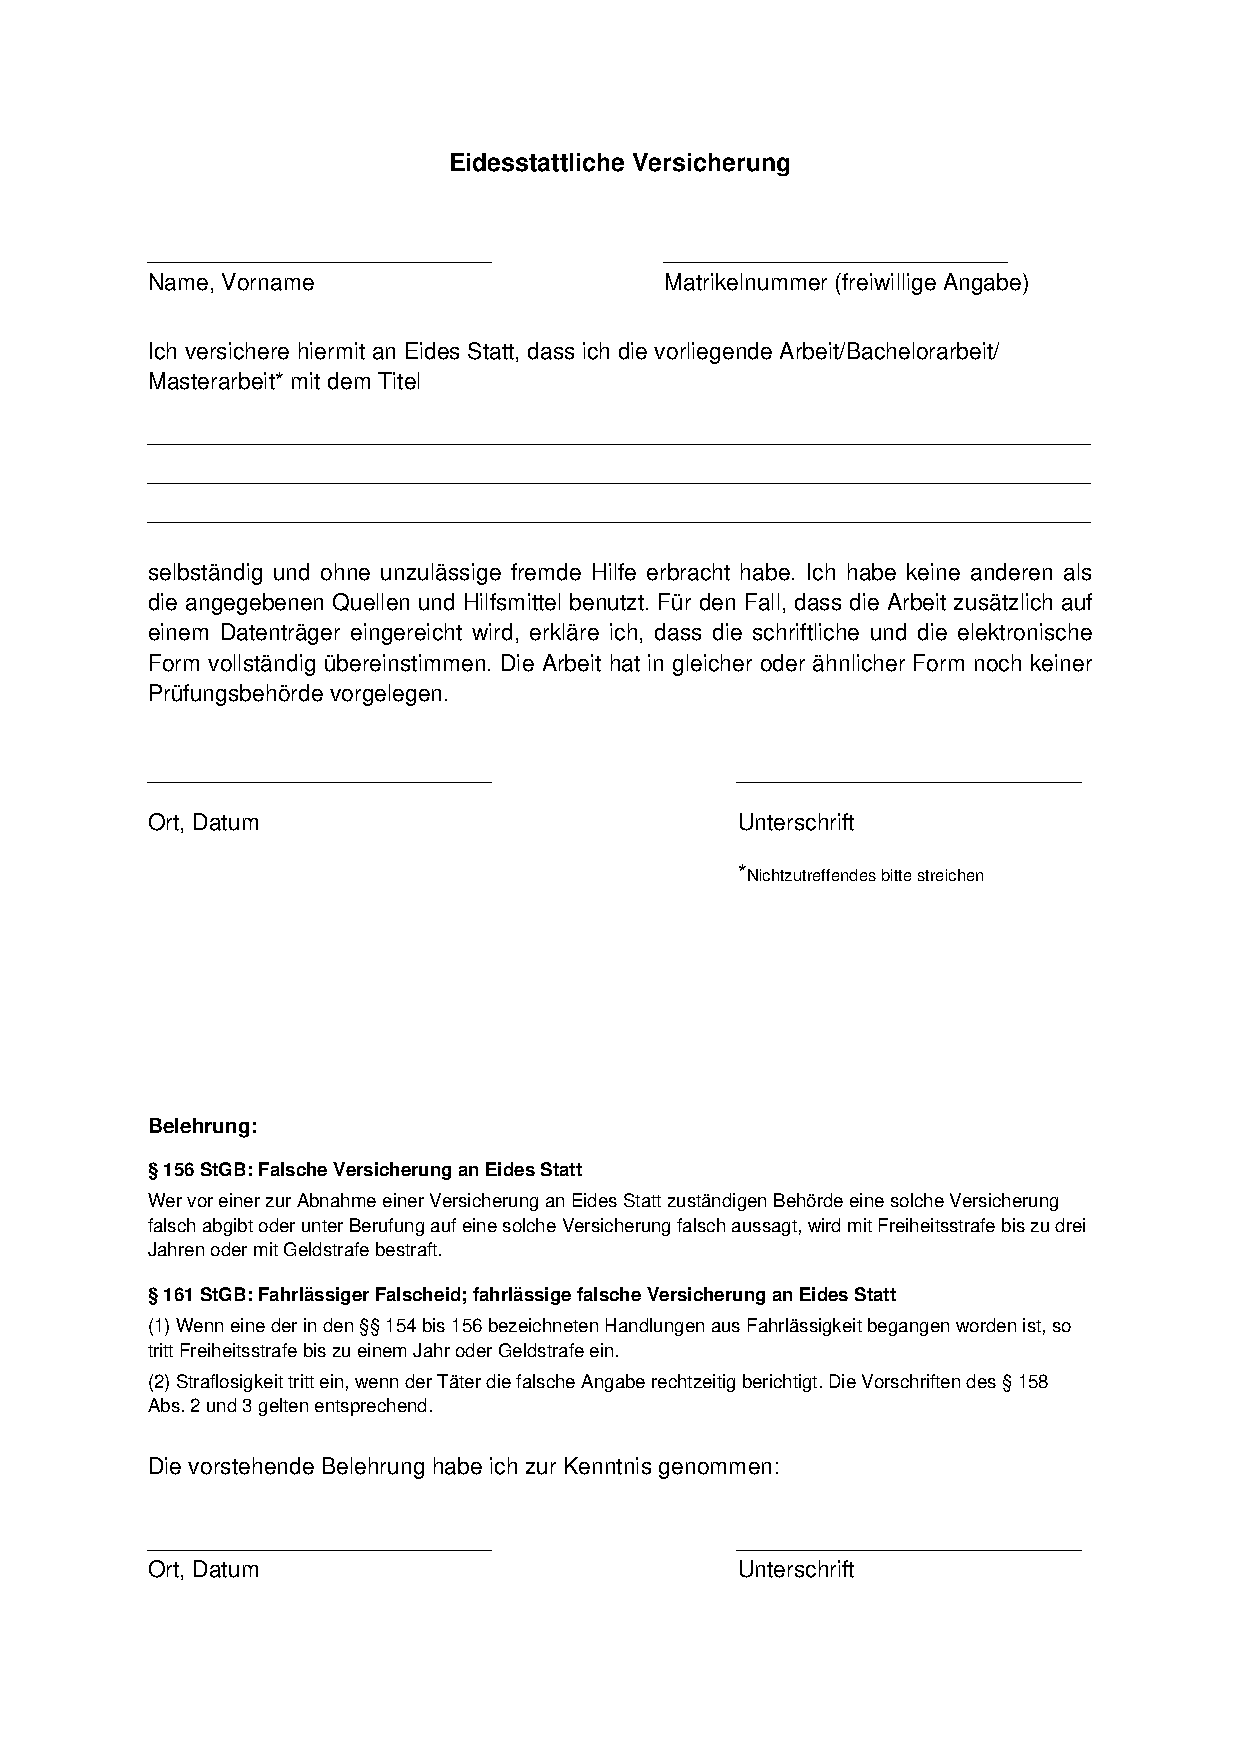
\includepdf[pages={1},offset=-1in -1in]{Formular_Eidesstattliche_Versicherung_neu.pdf}
 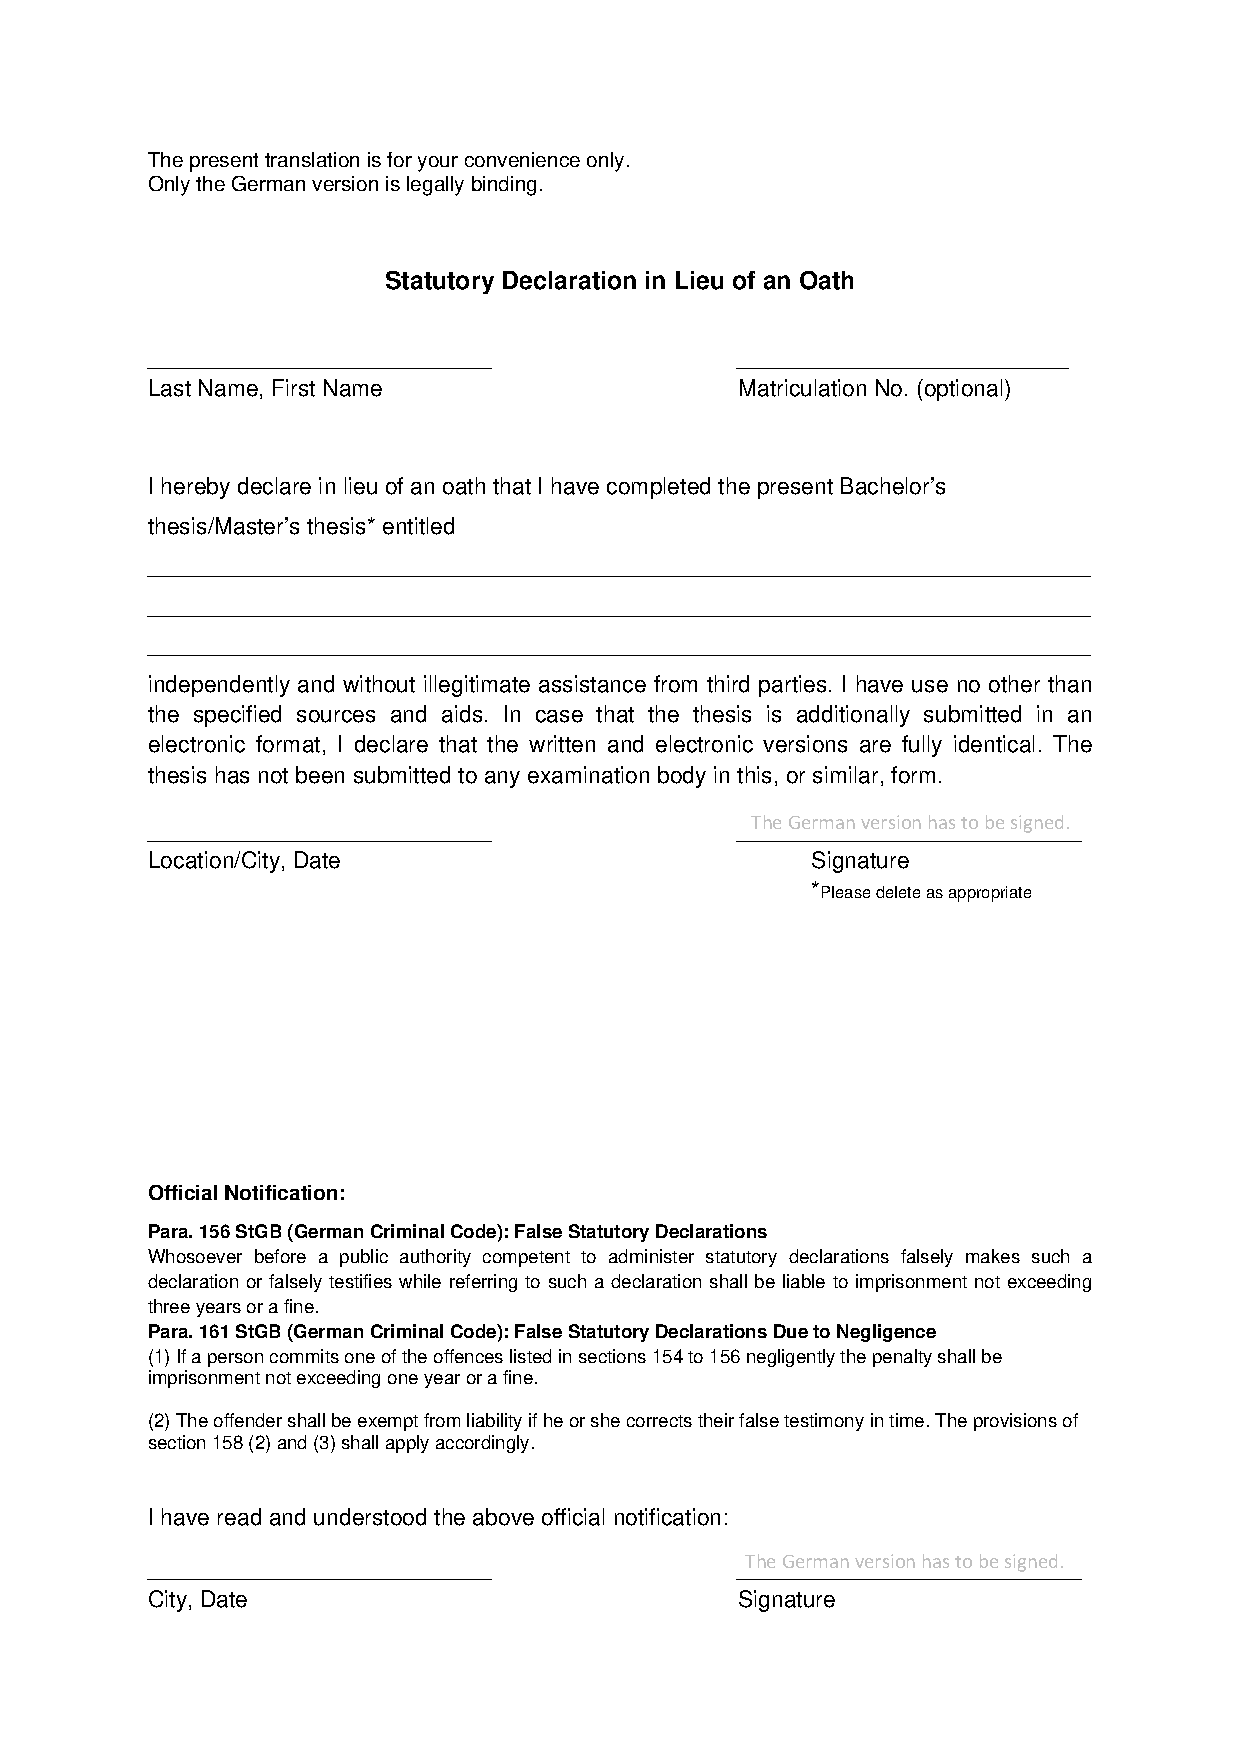
\includepdf[pages={1},offset=-1in -1in]{Statutory_Declaration_in_Lieu_of_an_Oath.pdf} % English 

\clearpage

%TODO rewrite
{\bf\Large Abstract} \\ [1em]
The topic of autonomous driving using artificial intelligence increases in importance with the overwhelming amount of software usage within vehicles. For that \textit{Convolutional Neural Networks} (CNNs), which try to figure out the importance of special areas of a single picture, have been shown to be promising. \\
In this paper we will give a general introduction to the topic of \nns and then state the specialties defining a CNN.
We distinguish between the three main paradigms currently used and researched for autonomous driving agents: mediated perception, behavior reflex and direct perception.\\
Further we will compare different domain specific languages \cnnarch, \caffe, \caffetwo and \mxnet, based on the factors of usability, scope of functionality, also regarding training possibilities, and the integration on a subject.

We will analyze a CNN using the direct perception approach, in different languages, and compare it to state-of-the-art implementations of the other paradigms, training on a simulator \torcs or the \kitti database. Furthermore we state scenarios probably causing problems for the direct perception approach. 

Finally we create an overview of the mentioned languages with a table, which states the functionalities and properties in a nutshell.
\cleardoublepage


%\vspace*{2cm}
{\bf\Large Aufgabenstellung}

\cleardoublepage


\tableofcontents

\clearpage

% Ab erstem Kapitel Seiten arabisch zählen
\setcounter{page}{1}
\pagenumbering{arabic}

%\chapter{Introduction}



\chapter{Preliminaries}

The field of autonomous driving agents has rapidly become a key factor in modern car manufacturing. Current research topic rises the agents from parking or lane keeping assistants to fully autonomous driving agents obeying the traffic rules and having the ability to react to the volatile environment in a reasonable way.

For that machine learning techniques have proven themselves as an essential part. In order to fulfill the security standards and create a sophisticated agent, it has to be trained on hundred-thousands of scenarios each having a large set of data attached, for example sensor and image data of multiple cameras.\\
The approach of \textit{Convolutional Neural Networks} (CNNs) have been proven to be powerful enough to handle this amount of training iterations with a huge number of input variables, while maintaining a large learning capacity. \cite{krizhevsky2012imagenet}

%In \Cref{chapter: DLL} we see that there is the need of specific languages for the design and implementation of such nets. We introduce four languages. Three are well known and established in the world of DSL and one is an upcoming new language.

%A CNN, as explained in \Cref{sec:CNN}, has a general structure, but can be altered, to fit into the approach, in various ways, influencing the result. Therefore we introduce in \Cref{chapter: Deep Learning Approaches} the three main approaches of using a CNN in the stated topic.
\section{Neural Networks}\label{sec: NN}

The \nns are a construct, adapted from biological processes. Its general structure is uncomplicated, but has immense expressiveness. The complete spectrum of what can be modeled by \nns is currently not known.\\
A neural net is made out of neurons and has one very basic function:\\
It takes a fixed number $n \in \mathbb{N}$ of the incoming values $x_i$, where the vector $(x_0,\dots x_n)^T$ is called a tensor, and multiplies them each with a specific weight $w_i$, where $0 \le i \le n$.
Also every neuron contains a bias $b$, which is a general value subtracted from the sum, so $\sum_{i=0}^{n} (x_i \cdot w_i) -b$. 

Often one applies an activation function to fix the value between 0 and 1. Such a function would be for example the sigmoid function, which is a non-linear functions. Without using a non-linear function one gets restricted to linear regression and therefore reduces their ability to model more complex functions. \cite{glorot2010understanding}
This non-linear normalized value gets forwarded to the neurons of the next layer.

Those neurons are ordered in different layers, visualized in \Cref{fig: Simple NN}.
\begin{enumerate}
	\item input layer (green):\\ \label{item input layer}
	This layer gets fed with the input values of the problem, which can be for example sensor data or pixel color values.
	\item hidden layer (blue):\\\label{item hidden layer}
	The hidden layer consists of neurons receiving the values from the previous layer, while not being obliged to have the same number of neurons (c.f. \Cref{fig: Simple NN}).
	Different architectures can be distinguished to be deep (c.f. \Cref{fig: Deep Neural Net}). This means, that there are multiple hidden layers of neurons instead of just one. The number of neurons a layer contains is again independent of the previous layers.\\
	Also for the hidden layers, it is possible to be not fully connected (c.f. \Cref{fig: not fullyconnected Neural Net}). Thus some neurons don't forward their value to every neuron of the next layer.\\
	There is no rule dictating the best architecture, considering number of layers, neurons per layer or the connectivity.
	\item output layer (yellow):\\ \label{item output layer}
	The output neurons produce the value of the \nn. Depending on the \nns purpose it can be for example a confidence value of a classification, like recognizing a stop sign, or the value of changing the steering wheel angle. 
\end{enumerate}

In order to train a \nn one has to define the behavior the \nn should have. In an image classification example, one should know what the correct class of a given image of a sign is, i.e. a speed limit sign. Those are called labels.\\
A \nn can then be trained by giving it values for the input layer and comparing the values of the output layer with the solutions it should have resulted in. The difference can then be checked. Such a difference can be simply \texttt{true}/\texttt{false} or a value indicating how big the difference is.\\
In the example of signs: a classification of a ``speed limit 70''-sign as a ``speed limit 50''-sign is still wrong, but not as bad as the classification as a ``stop''-sign.\\
Using this difference values, the \nn can use backpropagation, which is applied linear algebra, to adjust the weights $w_i$ and biases $b$ to improve the output iteratively.

Further information about the underlying training algorithms like gradient descent, newtons method, conjugate gradient or Levenberg-Marquardt algorithm is not given here in order to keep the paper in a justifiable length.  

\begin{figure}
	\centering
	\tikzset{input/.style = {ellipse,draw,fill=green!50!white, initial, initial text =}}
	\tikzset{hidden/.style = {ellipse,draw,fill=blue!50!white}}
	\tikzset{output/.style = {ellipse,draw,fill=yellow!50!white}}
	\begin{subfigure}[b]{0.25\textwidth}
	\begin{tikzpicture}[node distance = .5cm, on grid,auto]		
		\node[input] (i1) {};
		\node[input, below = of i1] (i2) {};
		\node[input, below = of i2] (i3) {};
		
		\node[hidden, above right = .25cm and 1cm of i1] (h1) {};
		\node[hidden, below = of h1] (h2) {};
		\node[hidden, below = of h2] (h3) {};
		\node[hidden, below = of h3] (h4) {};
		
		\node[output , right = 1cm of h2] (o1) {};
		\node[output , below = of o1] (o2) {};
		\coordinate[right = of o1] (c1) {};
		\coordinate[right = of o2] (c2) {};
		
		\path[->] (i1.east) edge (h1.west)
					(i1.east) edge (h2.west)
					(i1.east) edge (h3.west)
					(i1.east) edge (h4.west);
		\path[->] (i2.east) edge (h1.west)
					(i2.east) edge (h2.west)
					(i2.east) edge (h3.west)
					(i2.east) edge (h4.west);
		\path[->] (i3.east) edge (h1.west)
					(i3.east) edge (h2.west)
					(i3.east) edge (h3.west)
					(i3.east) edge (h4.west);
		\path[->] (h1.east) edge (o1.west)
				  (h2.east) edge (o1.west)
				  (h3.east) edge (o1.west)
				  (h4.east) edge (o1.west);
		\path[->] (h1.east) edge (o2.west)
					(h2.east) edge (o2.west)
					(h3.east) edge (o2.west)
					(h4.east) edge (o2.west);
		\path[->] (o1) edge (c1)
				  (o2) edge (c2);		
	\end{tikzpicture}	
	\caption{}
	\label{fig: Simple NN}
	\end{subfigure}
	\begin{subfigure}[b]{0.40\textwidth}
	\begin{tikzpicture}[node distance = .5cm, on grid,auto]		
	\node[input] (i1) {};
	\node[input, below = of i1] (i2) {};
	\node[input, below = of i2] (i3) {};
	
	\node[hidden, above right = .25cm and 1cm of i1] (h11) {};
	\node[hidden, below = of h11] (h21) {};
	\node[hidden, below = of h21] (h31) {};
	\node[hidden, below = of h31] (h41) {};
	
	\node[hidden, above right = .5cm and 1cm of h11] (h12) {};
	\node[hidden, below = of h12] (h22) {};
	\node[hidden, below = of h22] (h32) {};
	\node[hidden, below = of h32] (h42) {};
	\node[hidden, below = of h42] (h52) {};
	\node[hidden, below = of h52] (h62) {};
	
	\node[right =0.5cm of h12] (d1) {\dots};
	\node[below = of d1] (d2) {\dots};
	\node[below = of d2] (d3) {\dots};
	\node[below = of d3] (d4) {\dots};
	\node[below = of d4] (d5) {\dots};
	\node[below = of d5] (d6) {\dots};
	
	\node[hidden, right = 0.5cm of d1] (h13) {};
	\node[hidden, below = of h13] (h23) {};
	\node[hidden, below = of h23] (h33) {};
	\node[hidden, below = of h33] (h43) {};
	\node[hidden, below = of h43] (h53) {};
	\node[hidden, below = of h53] (h63) {};
	
	\node[output , right = 1cm of h33] (o1) {};
	\node[output , below = of o1] (o2) {};
	\coordinate[right = of o2] (c1) {};
	\coordinate[right = of o1] (c1) {};
	
	\path[->] (i1.east) edge (h11.west)
				(i1.east) edge (h21.west)
				(i1.east) edge (h31.west)
				(i1.east) edge (h41.west);
	\path[->] (i2.east) edge (h11.west)
				(i2.east) edge (h21.west)
				(i2.east) edge (h31.west)
				(i2.east) edge (h41.west);
	\path[->] (i3.east) edge (h11.west)
				(i3.east) edge (h21.west)
				(i3.east) edge (h31.west)
				(i3.east) edge (h41.west);
	\path[->] (h11.east) edge (h12.west)			
				(h11.east) edge (h22.west)
				(h11.east) edge (h32.west)
				(h11.east) edge (h42.west)
				(h11.east) edge (h52.west)
				(h11.east) edge (h62.west);
	\path[->] (h21.east) edge (h12.west)			
				(h21.east) edge (h22.west)
				(h21.east) edge (h32.west)
				(h21.east) edge (h42.west)
				(h21.east) edge (h52.west)
				(h21.east) edge (h62.west);
	\path[->] (h31.east) edge (h12.west)			
				(h31.east) edge (h22.west)
				(h31.east) edge (h32.west)
				(h31.east) edge (h42.west)
				(h31.east) edge (h52.west)
				(h31.east) edge (h62.west);			
	\path[->] (h41.east) edge (h12.west)			
				(h41.east) edge (h22.west)
				(h41.east) edge (h32.west)
				(h41.east) edge (h42.west)
				(h41.east) edge (h52.west)
				(h41.east) edge (h62.west);
					
	\path[->] (h13.east) edge (o1.west)
				(h23.east) edge (o1.west)
				(h33.east) edge (o1.west)
				(h43.east) edge (o1.west)
				(h53.east) edge (o1.west)
				(h63.east) edge (o1.west);		
	\path[->] (h13.east) edge (o2.west)
				(h23.east) edge (o2.west)
				(h33.east) edge (o2.west)
				(h43.east) edge (o2.west)
				(h53.east) edge (o2.west)
				(h63.east) edge (o2.west);		
	\end{tikzpicture}
	\caption{}
	\label{fig: Deep Neural Net}
	\end{subfigure}	
	\begin{subfigure}[b]{0.32\textwidth}
		\begin{tikzpicture}[node distance = .5cm, on grid,auto]		
		\node[input] (i1) {};
		\node[input, below = of i1] (i2) {};
		\node[input, below = of i2] (i3) {};
		
		\node[hidden, above right = .25cm and 1cm of i1] (h11) {};
		\node[hidden, below = of h11] (h21) {};
		\node[hidden, below = of h21] (h31) {};
		\node[hidden, below = of h31] (h41) {};
		
		\node[hidden, above right = .5cm and 1cm of h11] (h12) {};
		\node[hidden, below = of h12] (h22) {};
		\node[hidden, below = of h22] (h32) {};
		\node[hidden, below = of h32] (h42) {};
		\node[hidden, below = of h42] (h52) {};
		\node[hidden, below = of h52] (h62) {};
		
		
		\node[output , right = 1cm of h32] (o1) {};
		\node[output , below = of o1] (o2) {};
		\coordinate[right = of o2] (c1) {};
		\coordinate[right = of o1] (c1) {};
		
		\path[->] (i1.east) edge (h11.west)
			(i1.east) edge (h21.west)
			(i1.east) edge (h31.west)
			(i1.east) edge (h41.west);
		\path[->] (i2.east) edge (h11.west)
			(i2.east) edge (h21.west)
			(i2.east) edge (h31.west)
			(i2.east) edge (h41.west);
		\path[->] (i3.east) edge (h11.west)
			(i3.east) edge (h21.west)
			(i3.east) edge (h41.west);

		\path[->] (h11.east) edge (h12.west)			
			(h11.east) edge (h22.west)
			(h11.east) edge (h32.west);
		\path[->] (h21.east) edge (h22.west)
			(h21.east) edge (h32.west)
			(h21.east) edge (h42.west)
			(h21.east) edge (h12.west);
		\path[->] (h31.east) edge (h32.west)
			(h31.east) edge (h42.west)
			(h31.east) edge (h52.west)
			(h31.east) edge (h62.west);			
		\path[->] (h41.east) edge (h42.west)
			(h41.east) edge (h52.west)
			(h41.east) edge (h62.west);
		\path[->] (h12.east) edge (o1.west)
			(h22.east) edge (o1.west)
			(h52.east) edge (o1.west)
			(h62.east) edge (o1.west);		
		\path[->] (h12.east) edge (o2.west)
			(h22.east) edge (o2.west)
			(h32.east) edge (o2.west)
			(h42.east) edge (o2.west)
			(h52.east) edge (o2.west)
			(h62.east) edge (o2.west);		
		\end{tikzpicture}
		\caption{}
		\label{fig: not fullyconnected Neural Net}
	\end{subfigure}
	% das Dritte ist wenig Sinvoll vom Aufbau her
\end{figure}


\section{Convolutional Neural Network (CNN)}\label{sec:CNN}

A CNN is a special class of deep feed-forward \nns. One of the main design goals of a CNN is, that they require a minimal amount of preprocessing. This is an important aspect, because they are often fed with images. Preprocessing high resolution images is very costly in terms of computational time. In the context of autonomous driving the time is even more crucial, since the driving agent needs to be able to react to spontaneous events.

Like most parts of \nns, also the CNNs are inspired by biological processes. It is mainly based on the connectivity pattern of an animals visual cortex, where special neurons respond only to stimuli of their receptive field, represented as rectangles lying in the image. Partial overlapping guarantees a complete coverage of the field of view. Those rectangles are often called kernel, feature or filters.\cite{matsugu2003subject}

%The partitioning into those rectangles can also have the advantage, that the size of the input image is not relevant. If there would be a direct correspondence of a pixel to one input value then a change of the size would infer null values or additional input values, where the weights are not directly well suited. But with partitioning it into sub-rectangles of the image the values can be unified by selecting these rectangles relative to the size.
%This is only given, if there are no fully connected layers. Otherwise one has to perform other steps like cropping, scaling or padding. %TODO ref

%Using the so called pooling the net reduces the amount of inputs by mapping a number of values, for example the color values of a kernel, to one single value. One often used pooling type is the max pooling, which takes the maximal value of a property. Using pooling and relative sizes of kernels one can avoid the necessity of equally sized images. \cite{wiki:CNN} 
The four basic layer types, which are mostly used for CNNs are:
\begin{enumerate}
\setlength{\itemindent}{-0.5cm}
\item fully-connected layers:\\
	equal to the fully connected layers described for \nns (c.f. \Cref{sec: NN})
\item convolutional layers:\\
	A convolutional layer compares the given image with a list of features, the net thinks are key factors to indicate a certain item. In this context it could be an other car driving ahead of the host. Those features are not a-priori given, but learned by the CNN. \\
	It is simple to understand using an example:\\
	\begin{figure}[H]
		\centering
		\begin{tikzpicture}[node distance = .5cm]
		\node(table1) {\begin{tabular}{|c|c|c|c|} \hline
			7 & 6 & 5 & 5 \\\hline
			6 & 9 & 1 & 3 \\\hline
			4 & 1 & 2 & 8 \\\hline
			2 & 9 & 3 & 1 \\\hline
		\end{tabular}};
		\node[right = of table1](plus) {$\oplus$};
		\node[right = of plus](kernel) {\begin{tabular}{|c|c|} \hline
			-1 & 2 \\\hline
			2 & 0 \\\hline
		\end{tabular}};
		\node[right = of kernel] (equals){$=$};
		\node[right = of equals] (result) {\begin{tabular}{|c|c|c|} \hline
			17 & 22 & 7\\\hline
			20 & -5 & 9\\\hline
			2 & 21 & 20\\\hline
		\end{tabular}};
	
	
		\draw [red,ultra thick,rounded corners] (-1.25,1) rectangle (0,0);
		\draw [green!75!black,ultra thick,rounded corners] (-0.6,0.5) rectangle (0.6,-0.5);
		
		\draw [red,ultra thick,rounded corners] (3.05,0.55) rectangle (4.45,-0.55);
		\draw [green!75!black,ultra thick,rounded corners] (3.0,0.6) rectangle (4.5,-0.6);
		
		\draw [red,ultra thick,rounded corners] (6.25,0.75) rectangle (7.1,0.25);
		\draw [green!75!black,ultra thick,rounded corners] (7.1,0.25) rectangle (7.9,-0.25);
		
		\end{tikzpicture}
	\end{figure}
	The left most is the input and the second one is the kernel. The result is computed as a piece-wise multiplication and then adding them up. The convolution can differ in kernel size and stride, which denotes the movement of the kernel. In the example we have a kernel of size $2\times2$ and a stride of 1.\\
	So for example (red case): $7\cdot(-1)+\cdot6\cdot2+\cdot6\cdot2+4\cdot0=17$\\
	The number now represents the similarity or likelihood of the feature to be in that position. Edge detection can be applied easily using such a layer. \cite{hubel1968receptive}
\item rectified linear units (ReLUs):\\
	Those ReLUs perform a normalization step, by applying the function $max(0,x)$ to every element $x$. So for the example:
	\begin{figure}[H]
		\centering
		\begin{tabular}{|c|c|c|} \hline
			17 & 22 & 7\\\hline
			20 & -5 & 9\\\hline
			2 & 21 & 20\\\hline
		\end{tabular}
		$\Rightarrow$
		\begin{tabular}{|c|c|c|} \hline
			17 & 22 & 7\\\hline
			20 & 0 & 9\\\hline
			2 & 21 & 20\\\hline
		\end{tabular}
	\end{figure}
	The main purpose of such a ReLU is to create the prerequisite of mathematical functions, only accepting non-negative values. Often times researchers tend to use the function $ln(1+e^x)$ in order to have a differentiable approximation of ReLU. 
\item pooling layers:\\
	The pooling layer reduces the input by having a windows size, which is typically 2 or 3, and a stride, which is typically 2, and map the values within the window to one single value. In our example this is done using the maximum value.
	\begin{figure}[H]
		\centering
		\begin{tikzpicture}[node distance = .5cm]
		\node (input) {\begin{tabular}{|c|c|c|} \hline
			17 & 22 & 7\\\hline
			20 & 0 & 9\\\hline
			2 & 21 & 20\\\hline
		\end{tabular}};
		\node[right = 0.7cm of input] (arrow) {$\Rightarrow$};
		\node[right = of arrow] (result) {\begin{tabular}{|c|c|} \hline
			22 & 9 \\\hline
			21 & 20\\\hline
		\end{tabular}};
	
		\draw [red,ultra thick,rounded corners] (-1.25,0.8) rectangle (0.4,-0.3);
		\draw [green!75!black,ultra thick,rounded corners] (0.41,0.8) rectangle (2.06,-0.3);
		
		\draw [red,ultra thick,rounded corners] (3.32,0.5) rectangle (4.12,0);
		\draw [green!75!black,ultra thick,rounded corners] (4.16,0.5) rectangle (4.96,0);
		\end{tikzpicture}
	\end{figure}
	For the red case, the value 22 is the maximum of the window containing $\{17,22,20,0\}$. For the green case, the 9 calculated is the maximum of the window $\{7,9\}$ since through a stride of 2 the window in partially not contained in the input.
\end{enumerate}

The application of convolution and pooling has the advantage that it reduces the effort to train a CNN. The weights and biases of neurons of each receptive field are equal. This is reasonable since for example a speed limit road sign should be identified independent, whether it is located next to the road, like on a normal road, or above the road, like on an highway. \cite{lecun2015lenet}

%Further CNNs make strong and mostly correct assumptions about the nature of images, like stationary of statistics and locality of pixel dependencies. This leads to fewer connections and parameters, compared to a normal feed-forward neural net with similar sized layers, and therefore reduces the time it takes to be trained, while being only slightly worse in their best-performance. \cite{krizhevsky2012imagenet}

\section{AlexNet} \label{sec: AlexNet}

The \textit{\alexnet} was one of the best performing CNN architectures in 2012 and is still performing good enough to be used for various problems. It was originally trained on the ImageNet subsets of \texttt{ILSVRC-2010} and \texttt{ILSVRC-2012} \footnote{Further information: http://www.image-net.org/challenges/LSVRC/} and became famous, because of its result being way ahead of all other competitors.

A highly optimized GPU implementation of this architecture combined with innovative features is publicly available. Those features lead to improve performance and reduce training time.\cite{krizhevsky2012imagenet}

An important note is that the original test is dated back to 2012 and therefore was used with an overall GPU memory of 6 GB, with which training took about six days. With modern hardware like new GPUs, SLI usage (having multiple GPUs) or even clusters, the training can be done faster, or the model can be trained with more data to improve performance. The improvement caused only by hardware can be roughly grasped through \cite{sze2017hardware}.

%\todo{maybe calc the possible speed up based on ``Hardware for Machine Learning''}

\begin{figure}[ht]
	\centering
%	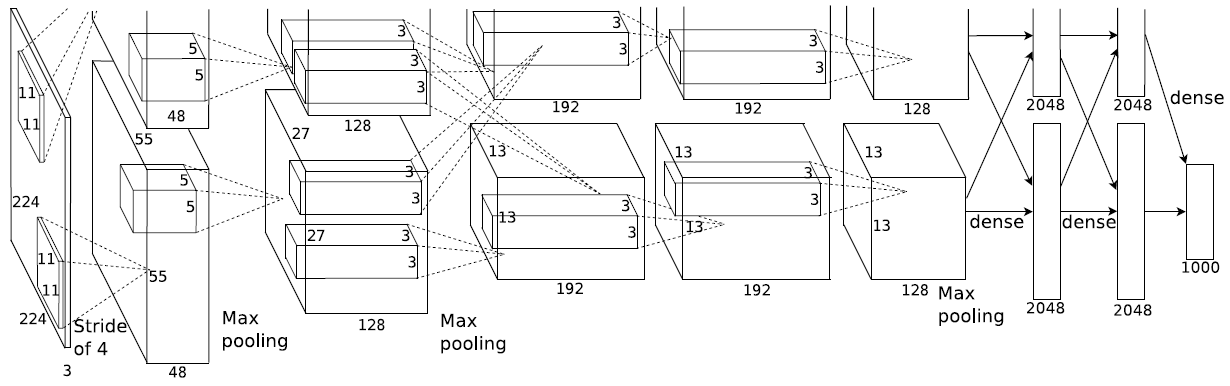
\includegraphics[scale = 0.45]{src/pic/AlexNet-structure.PNG}
	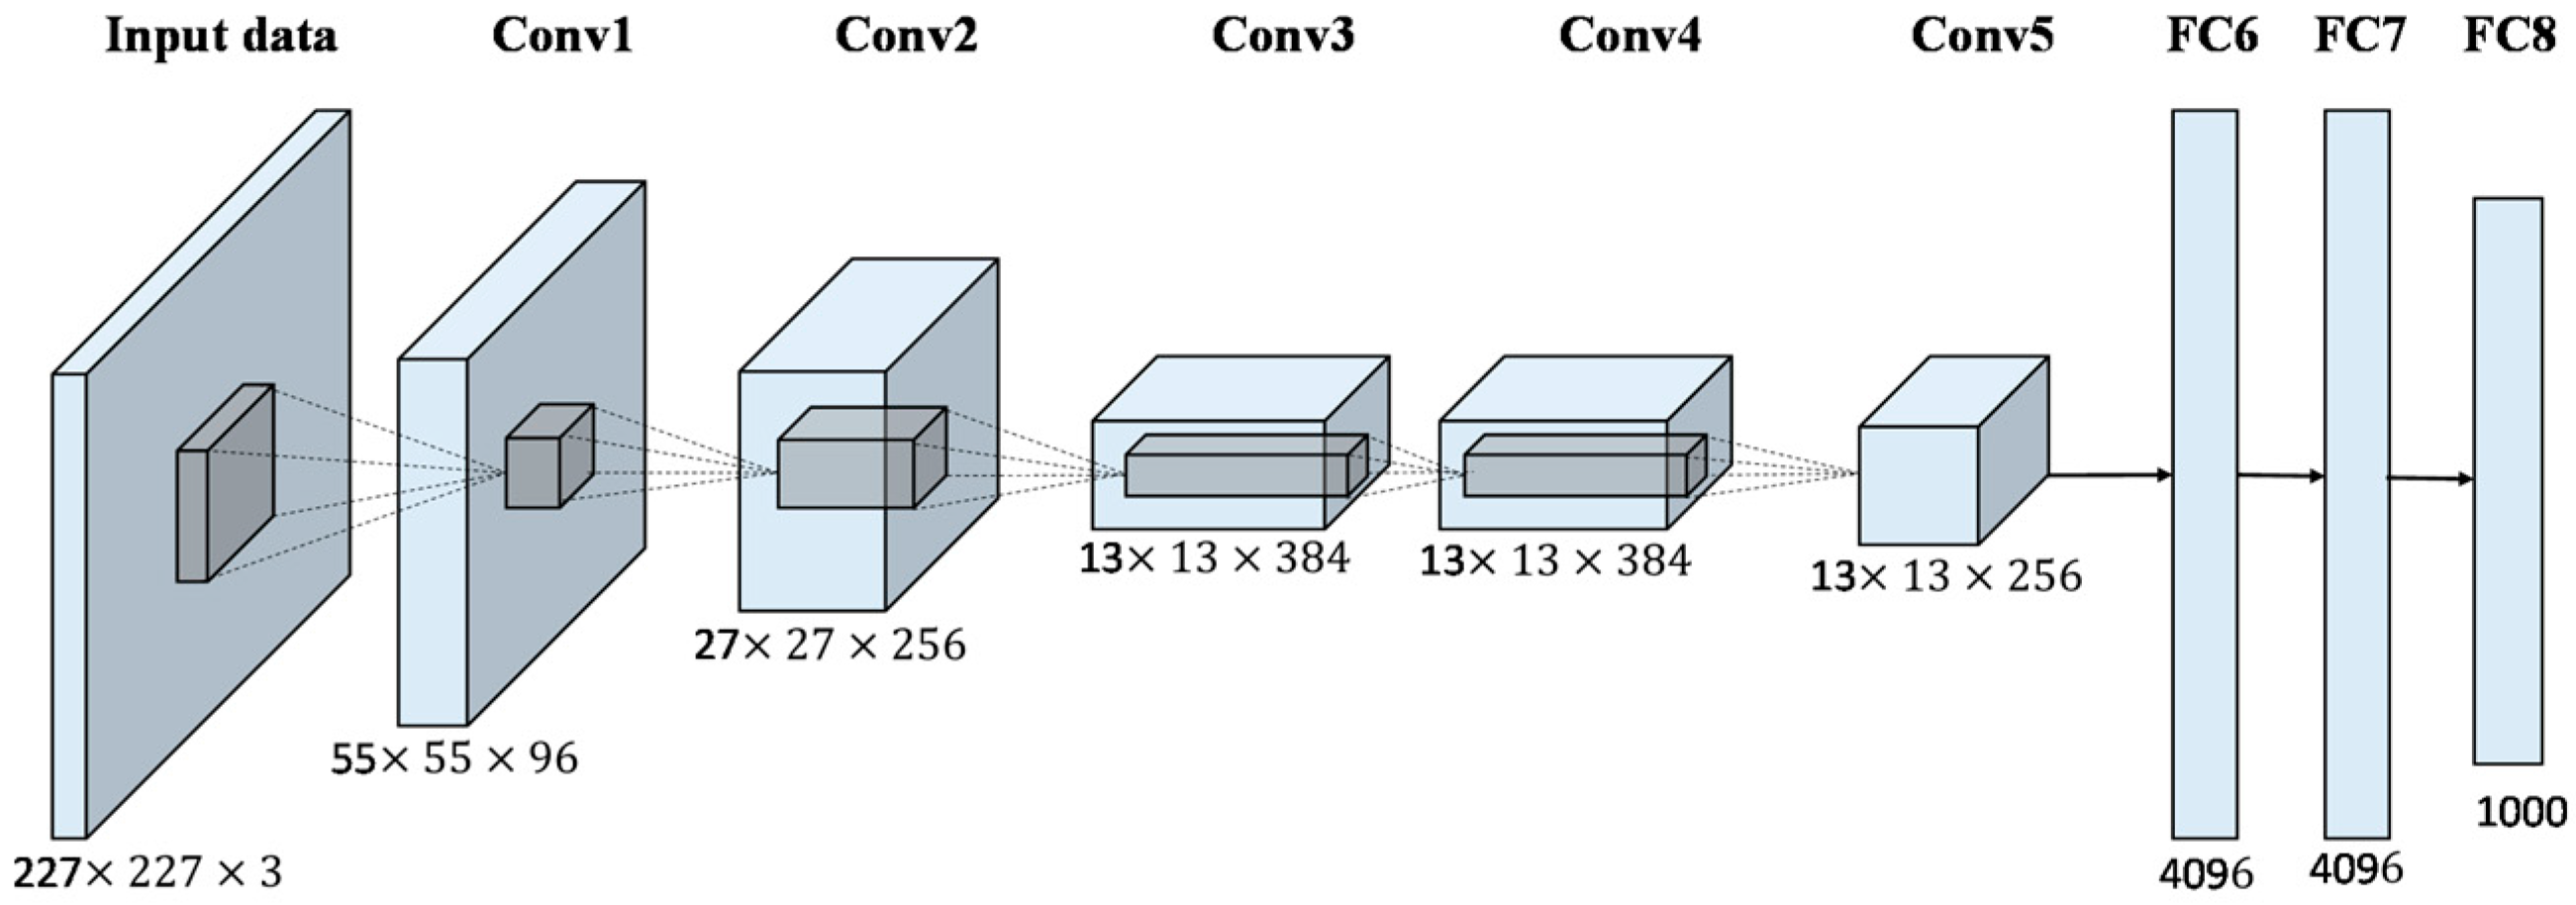
\includegraphics[scale = 1.3]{src/pic/AlexNet-structure-simple.PNG}
	\caption{The \alexnet-architecture. It consists of 5 convolutional layers (at the beginning), and three fully-connected layers (at the end). \cite{han2017pre}
	\cite{krizhevsky2012imagenet}}
	\label{pic: AlexNet}
	%TODO redraw in simple
\end{figure}

\chapter{Deep Learning Languages}\label{chapter: DLL}

Constructing a CNN from scratch in any typical language like Java, C++, or Python is very elaborately and has a high error potential. Even libraries in any such language often encounter the problem of over-complication due to their own style and syntactical and semantic architecture. Therefore there is a need of specialized languages.

The Deep Learning Languages (DLLs) are part of the Domain Specific Languages (DSL). Their main goal is to provide an easy to understand, as less verbose but as expressive as possible way of describing a CNN with its different layers and connections. Also one wants to have simple build pre-sets.

%SEE: maybe maintain the number
For that we consider three deep learning languages and analyse them on the previously mentioned properties.

\section{CNNArchLang}\label{sec: CNNArch}

(The whole description is based on\cite{CNNArch} and especially \cite{tim2018CNNArchLang})

One language for modeling CNNs is CNNArchLang. This language is developed at the Chair of Software Engineering, especially Thomas Michael Timmermanns,  at the RWTH Aachen University and part of the MontiCar language family. The main purpose of its creation is the necessity of special properties not given by other CNN-languages: \textit{C\&C integration} and \textit{type-safe component interface}. Its basic structure is very similar to python to improve understanding, based on familiarity with Python, and have an equal non-typed syntax. 

One very huge advantage of \cnnarch is that it's designed to be very simplistic and have less verbose than most other languages to model CNNs. It does so, by moving from defining a CNN by every single neuron to the definition via layers only. For that specific purpose many layers are already defined (c.f. \Cref{subsec: CNNArchLang - predefines layers}). 
New layers can be constructed by combining predefined layers.\\
This slightly reduces the expressiveness, since the possibility of performing computations on single tensors is lost. Such low-level operations are used extremely rarely and are not a drastic disadvantage.

In contrast to other languages for deep learning \cnnarch does not denote the connections of layers directly, but tries to model the data flow through the network. For that specific task it contains two main operators:
\begin{itemize}
	\item[-$>$:] Serial Connection:\label{item: sequential connection}\\
	This orders two elements sequentially. This means it denotes the first elements output as the second elements input. 
	\item[$|$:] Parallelization:\\
	This allows the split of the network into separate data streams, which can be computed in parallel.
\end{itemize}
Since serial connection has the higher precedence one has to use brackets. Also to merge the splitted streams, created by $|$, one can use the operators: \texttt{Concatenate()}, \texttt{Add()} and \texttt{Get(index)}.

\subsection{General Definitions}\label{subsec: general definitions}
The general definitions of a CNN, which are the input, i.e. an image, maybe additional data in a specific file type, i.e. sensor data, and the output dimension, denoting the predictions or in our example the actions the car should perform. Those are the only typed values within the CNN model.

Such definitions can be modeled in \cnnarch as presented in \Cref{lst: general definitons CNNArchLang}.

\begin{figure}[H]
	\centering
	\begin{lstlisting}
	def input Z(0:255)^{3, h, w} image[2]
	def input Q(-oo:+oo)^{10} additionalData
	def output Q(0:1)^{3} predictions
	\end{lstlisting}
	\caption{A general definition of a CNN using \cnnarch}
	\label{lst: general definitons CNNArchLang}
\end{figure}

Further analyzed the definition can be broken down to the following components:
\begin{itemize}
	\item Keyword: \texttt{def}\\
	Every input and output can be introduced using the keyword \texttt{def}
	\item Direction: \texttt{input}/\texttt{output}\\
	Every definition, being a part of the \ref{subsec: general definitions}, has to be defined to be either an \texttt{input} or an \texttt{output}
	\item Range of numbers:\\
	One can define the input to have special constraints. For example only integer values are denoted by a \texttt{Z} representing $\mathbb{Z}$. The same for \texttt{Q} and $\mathbb{Q}$. \\
	Also the range has to be given via \texttt{(x:y)}, where \texttt{x} and \texttt{y} either are numbers or \texttt{-oo}( or \texttt{oo}) to denote $\infty$.
	\item Size:\\
	The size of for example the input or the number of classes is denoted by a matrix like notation using \texttt{\^{}\{size\}}  . For the input image (line 1) the size \texttt{\^{}\{3,h,w\}} determines the input image to have 3 channels with an image width of \texttt{w} and image height of \texttt{h}.
	The others are just defined as 1$\times$10 or 1$\times$3 vectors/tensors.
	\item Naming:\\
	At the end of the line there has to be a name to identify the corresponding input/output.\\
	Also through the \texttt{[2]} behind the name \texttt{image} one can define it to be a fixed length array of images.
\end{itemize}

%\subsection{Array handling}
%An array, like in the example shown in \Cref{lst: general definitons CNNArchLang}, can be used either element wise:
%\begin{center}
%	\texttt{image[0]-$>$}
%\end{center}
%which would access the first image and create a sequential connection (c.f. \Cref{item: sequential connection}),
%whereas 
%\begin{center}
%	\texttt{image-$>$} $\equiv$ \texttt{(image[0] | image[1]) -$>$}
%\end{center}
%would result in two separate streams. If the receiving end of the sequential connection, for sake of example let it be called \texttt{out}, is also an array of size two one can also use
%\begin{center}
%	\texttt{image -$>$ out} $\equiv$  \texttt{([0]-$>$ out[0] | [1] -$>$ out[1])}
%\end{center}

\subsection{Predefined Layers and Functions} \label{subsec: CNNArchLang - predefines layers}
Different CNNs often use a similar basic set of layers, but arranging them differently. For that purpose there are some layers already defined by \cnnarch to simplify the usage.
There is for example the \texttt{FullyConnected}-layer with parameters for the number of units within and whether they should use a bias value (c.f. \Cref{sec: NN}), the \texttt{Convolutional}-2D-layer with parameters for the kernel (rectangle) size, number of filters, the stride defining the distance of two rectangles, padding and the usage of biases. Further information on any of these parameters or other predefined layers can be found in \cite{CNNArch}.

Also there are already defined functions like the \texttt{Sigmoid}, \texttt{Softmax}, \texttt{Tanh} or \texttt{ReLu}. 
One important aspect is that every argument has to be named. 

One important aspect is that \cnnarch is not a framework itself. It is used to create the code to function in the \mxnet (see \Cref{sec: MxNet}).
%\todo{\begin{itemize}
%\item talk about types and checks (4.4)
%\item not all CNNs since no low-level operators
%\item as expressive as Caffe but < MxNet
%\item less verbose than Caffe example of page 50(57)
%\end{itemize}}

\section{Caffe} \label{sec: Caffe}

%information based on \cite{jia2014caffe}

\caffe is a full deep learning framework, created by Yangqing Jia during hos PhD at UC Berkeley. It is a framework specially build to deal with multimedia input formats using state-of-the-art deep learning techniques. It comes as a BSD-license C++ library offering python and MATLAB bindings. One of its reasons why it's so well known and frequently used is because of its design based on expressiveness, speed and modularity.

Using Nvidias Deep Neural Network library cuDNN as a wrapper of the CUDA functionality, \caffe can use the GPU in order to process even faster and learn in a rate of 40 million pictures per day. The possibility of using multiple GPUs in SLI is not stated and therefore not taken into account. \cite{wiki:Caffe}
However the possibility of using a cloud system is mentioned. But whether it is a simple decentralization or the possibility to train the network using the combined power of multiple computers to train is not mentioned. \cite{jia2014caffe}

\caffe tries to improve its readability by abstracting from the actual implementation using a graph-oriented way of network defining. For that \caffe uses two elements to represent the network:
\begin{itemize}
	\item \textbf{Blob}:\\
		A 4-dimensional array storing data, like images, parameters or parameter updates. These blob are the communication between layers.
	\item \textbf{Layers}:\\
		A Layer as described in \Cref{sec: NN} and \Cref{sec:CNN}.
\end{itemize}
The whole model gets saved as a Google Protocol Buffer, which is a language-neutral structuration, with important key features like size-minimal and efficient serialization and efficient interfaces for C++ and Python. \cite{jia2014caffe} \cite{varda2008protocol}
An example of a graph and its corresponding Protocol Buffer representation, written in prototxt, are given in \Cref{fig: Caffe Graph and Protobuf}.


\begin{figure}
	\centering
\begin{subfigure}[b]{0.45\textwidth}
\begin{lstlisting}[basicstyle=\tiny]
name: "loss-net"
layers {
	name: "mnist"
	type: DATA
	top: "data"
	top: "label"
	data_param { ### }
}

layers {
	name: "ip"
	type: CONVOLUTIONAL
	bottom: "data"
	top: "conv"
	convolutional_param { ### }
}

layers {
	name: "loss"
	type: SOFTMAX_LOSS
	bottom: "ip"
	bottom: "label"
	top: "loss"
}
\end{lstlisting}
\caption{}
\label{lst: Google Protocol Buffer Example}
\end{subfigure}
\begin{subfigure}[b]{0.45\textwidth}
	\begin{tikzpicture}[every node/.style={draw, line width=0.5mm}, scale = 0.6]
		\node[rectangle, fill = blue!50] at (1,8) (mnist) {mnist(DATA)};
		\node[chamfered rectangle, draw, fill=yellow!75!orange] at (0,6) (data) {data};
		\node[chamfered rectangle, draw, fill=yellow!75!orange] at (5,4) (label) {label};
		
		\node[rectangle, fill = blue!50] at (0,4) (conv1) {ip(INNER\_PRODUCT)};
		
		\node[chamfered rectangle, draw, fill=yellow!75!orange] at (0,2) (conv) {ip};
		
		\node[rectangle, fill = blue!50] at (1,0) (loss) {loss({\footnotesize LOSS\_TYPE})};
		
		\path[->, thick] (mnist) edge (data);
		\path[->, thick] (mnist) edge (label);
		\path[->, thick] (data) edge (conv1);
		\path[->, thick] (conv1) edge (conv);		
		\path[->, thick] (conv) edge (loss);
		\path[->, thick] (label) edge (loss);
	\end{tikzpicture}
	\caption{}
	\label{fig: Caffe Graph Example}
\end{subfigure}
\caption{An example of a Softmax loss network. Blue boxes are the different layers and the yellow boxes are the blobs. Note that in (a) the parameters are not mentioned since they do not add value to this example. There are things defined like kernel size, image scaling or image origin.}
\label{fig: Caffe Graph and Protobuf}
\end{figure}

The biggest advantage of \caffe is the huge community providing a large set of presets, like layers or pre-trained nets and also a huge forum to ask other users about problems regarding ones project. This is such an advantage, because every module it is  guaranteed to pass a coverage test. \cite{jia2014caffe}

\caffe is written using as plaintext named prototxt and therefore can be run via command line. One problem mentioned with that is that even though there are many nets already defined the creation of new nets often is highly verbose and repetitive. There are no shortenings. For example \cite{tim2018CNNArchLang} mentioned an example net written in \cnnarch with 36 lines and in \caffe with 6700 lines. This is also due to the fact that even if a layer can be constructed as a composition of existing layers one often has to define the forward-, backward and gradient-updates. %TODO ref

\section{Caffe2} \label{sec: Caffe2}
The framework \caffetwo is the successor of \caffe. \caffetwo is developed by Facebook and its current main usage is the phrase-wise translation in social networks. Keeping the modulartiy of \caffe in mind \caffetwo is also designed so that it can be up-scaled as well as mobile deployed. Also \caffetwo is designed in such a fashion that it can easily adapt to drastic changes like quantized computing. \cite{Caffe2Homepage}

Since the whole architecture is rewritten from scratch and regarding its now roughly one year of existence the library performs relatively well, but does not have the impact to outperform \caffe \cite{heise:Caffe2}.
One upside of the rewriting is that \caffetwo has a Python binding, like most other frameworks. One downside of the rewriting is that huge parts of the framework are not sufficiently documented. \caffetwo tries to improve but still has large whole within the documentation. \cite{tim2018CNNArchLang}

\caffetwo offers programs, which allow the user to convert \caffe and PyTorch models to \caffetwo. This makes the switching to \caffetwo much easier, since the users don't have to rewrite their models. \cite{Caffe2Homepage}

The main difference between \caffe and \caffetwo in terms of designing a \nn is that in \caffetwo the user uses \texttt{Operators} as the basic units instead of layers. Even though they are similar to the layers of \caffe, they are more flexible and adaptable. Partly based on the popularity of \caffe, \caffetwo also has a huge community and a large set of preset \texttt{Operators}, which can be used. \cite{Caffe2Homepage}

%\section{Tensorflow} \label{sec: Tensorflow}

\section{MxNet}\label{sec: MxNet}

An other framework often mentioned in research is the \mxnet. This deep learning framework is part of the Apache Software Foundation. Also it is said to be ``Amazons deep learning framework of choice'' \cite{infoworld} and featured to be a preset on the Amazon Web Services (AWS). \cite{chenmxnet}

The \mxnet tries to combine the advantages of imperative frameworks like numpy or MatLab with the advantages of declarative frameworks like \caffe, \caffetwo or \tensorflow.

The advantages of imperative and declarative approaches can best be understood using an example.
Let the example be to compute: $a = b+c$
\begin{itemize}
	\item[] \textbf{imperative}:
		\begin{itemize}
			\setlength{\itemindent}{1.5cm}
			\item[Procedure:] check the ability of $b$ and $c$ to be added. If so strictly compute the sum and declare $a$ as the same type as $b$ and $c$
			\item[Advantage:] very straightforward, works well with typical structures, debugger and third party libraries
			\item[Usefull for:] natural parameter updates and interactive debugging
		\end{itemize}
	\item[] \textbf{declarative}:
		\begin{itemize}
			\setlength{\itemindent}{1.5cm}
			\item[Procedure:] compute the computation graph and store the values of $b$ and $c$ as data bindings
			\item[Advantage:] perform computation as late as possible, leading to good optimization possibilities
			\item[Usefull for:] specifying computation structure, optimization
		\end{itemize}
\end{itemize}

By combining both approaches \mxnet is able to provide a superset programming interface compared to \caffe. \cite{chen2015mxnet}

Also \mxnet is able to reduce memory to a minimum by performing everything they can in-place and free or reuse as fast as possible. Thus the memory usage of \mxnet is outperforming \caffe. \cite{chen2015mxnet} % and tensorflow
A new benchmark with \caffetwo has not been done yet.

An other very big upside of \mxnet is the possibility to use not only multiple GPUs in an SLI connection, but also multiple computers or even server to train a \nn simultaneously. This results in an outstanding scalability. \cite{chen2015mxnet}

Similar to \caffetwo, \mxnet also allows the deployment of trained models to low-end devices using Amalgamation (c.f. \cite{MxNetHomepage}) or the AWS.

Due to the fact that \mxnet has found its way into Apache Incubator and therefore it is an Open-Source project, the creation of additional functions and nets is quite simple and is not bound to a given preset. Thanks to the community also a variety of nets constructed and some already pre-trained are free to use. \cite{MxNetGithubModelGallery}


\chapter{Available Deep Learning Approaches}\label{chapter: Deep Learning Approaches}

There are various approaches of autonomous driving agents making a variety of assumptions and differ in numerous options. But they can be mostly categorized into two major groups of approaches: mediated perception approaches and behavior reflex approaches. \cite{chen2015deepdriving}

In this paper we further analyse a suggested third group, called direct perception, which can traced to \cite{gibson1979ecological} in the mid 50's, but was sharply criticized by researchers of the other two groups, i.e. in \cite{ullman1980against}. %TODO: fix 60's to be the first

All these three groups differ in the way of interpreting the given sensor data and whether or not to create a some what bigger picture based on consequent data.

\section{Mediated Perception} \label{sec: Mediated Perception}

The mediated perception approach is a multi-component continuous process. Every component recognizes specific aspects for driving. For example traffic signs, lanes, other cars. Those components are then combined into one single world state representing the cars surrounding based on the sensor data. \cite{KITTI}\\
These world states are 3D models of the current world. Cars are identified using a classifier and then often surrounded by a 3D bounding box. An example can be seen in \Cref{pic: 3D Bounding Box}. By comparing different frames generated one can estimate the speed and distance to those objects and derive an A.I. based precedence behavior. \cite{KITTI}\cite{chen2015deepdriving}

The often stated problems with such approaches are, that computing such a scene is costly in terms of computation time. Some information is irrelevant, redundant or even misleading due to inaccuracy of sensors. To perform a right turn the sensor information of the distance to a car left behind me is irrelevant, but becomes very important when taking a left turn.\\
Additionally many of the subtasks are still open research topics themselves. For example a reliable lane detection throughout various weather conditions or even a new road not having any drawn lines yet. \cite{aly2008real}\\
Also mediated perception approaches require very detailed information up front, like up-to-date maps.

The approach of mediated perception is a reasonable and very sturdy way of handling such a complex task, but has its drawbacks regarding computational time and additional knowledge.

\begin{figure}
	\centering
%	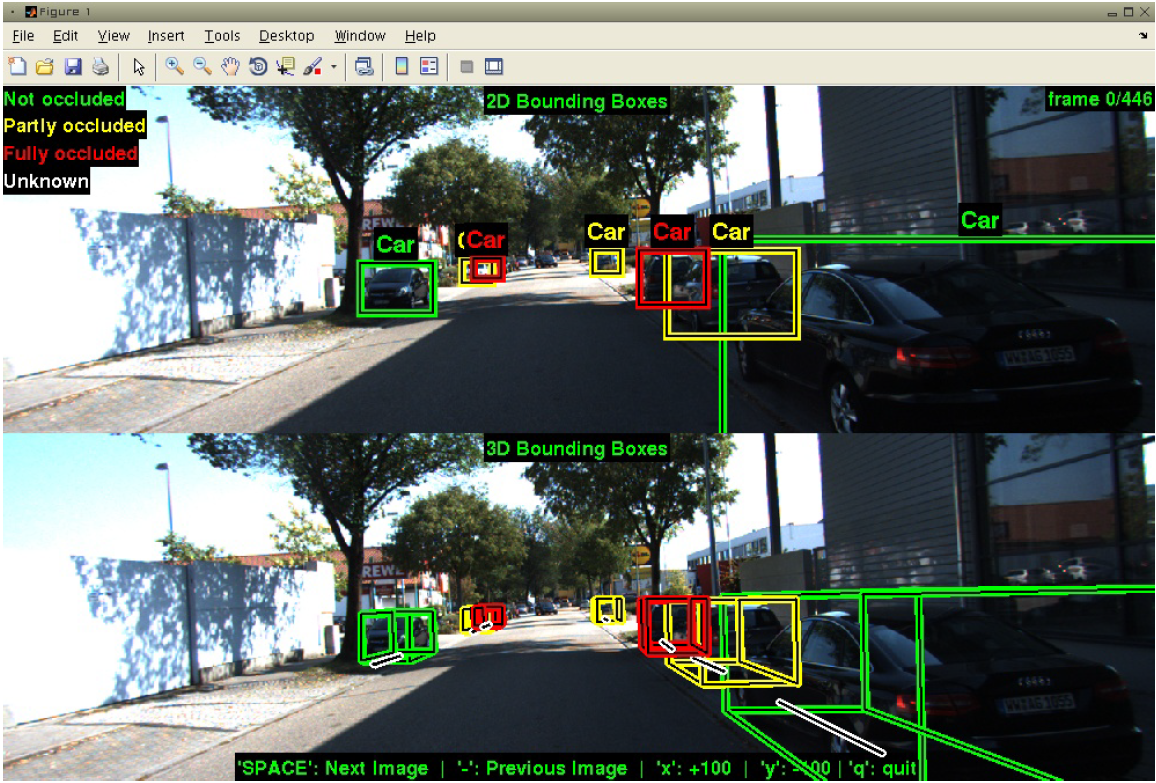
\includegraphics[scale=0.4]{src/pic/3D-boundingbox-example.png}
	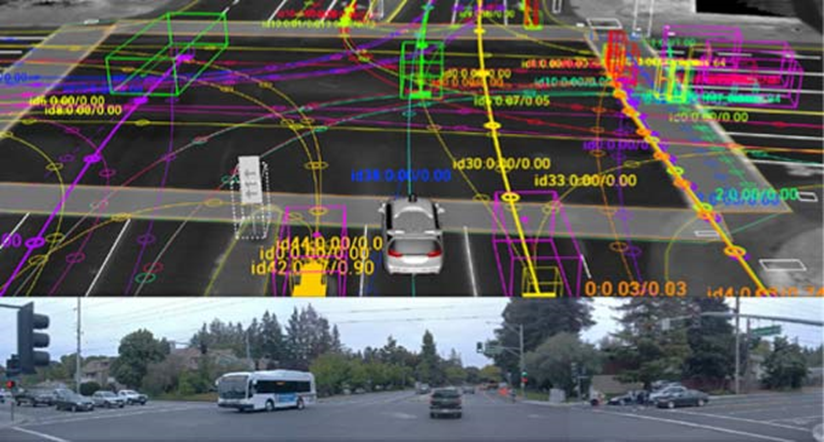
\includegraphics[scale=0.7]{src/pic/intersection.png}
	\caption{An example of a scene using 3D bounding boxes and path prediction.}
	\label{pic: 3D Bounding Box}
\end{figure}

\section{Behavior Reflex}\label{sec: Behavior Reflex}

The behavior reflex approach of constructing a reliable autonomous driving agent can be dated back to 1989 , where researchers tried to directly map a single frame to a decision of a steering angle. For such approaches a quite simple \nn was created. \\
The network \alvinn consisted of a single hidden layer, used back-propagation and is fed by two cameras: a $30\times32$ pixel video and a $8\times32$ pixel range finder retina. The input neurons fired depending on the blue color band of its pixel, because it is believed to infer the highest contrast between road and non-road. The difference in color of road and non-road was fed back to the network. The bias (activation level) is proportional to the proximity of the corresponding area, based on the likelihood and importance of having road in particular fields of the image.\cite{pomerleau1989alvinn}\\
For example having recognized that the road abruptly ends right in front of the car is more important than recognizing that there is a road in the top left corner.\\

Such systems, even though they are simple compared to the in \Cref{sec: Mediated Perception} mentioned mediated perception approaches, have been proven to have the capability to perform simple tasks. It can elegantly be trained by having a human drive a car with the cameras equipped and forward the images to the \nn and adding the current steering angles as a label.\cite{chen2015deepdriving}\\

The problem with behavior reflex approaches is, that they reach their limits very early when adding more complex scenarios. Having simple alternations to the trained scenarios, which enforce a different behavior, is very hard to train to such a \nn.\\
For example comparing a simple straight 3 lane road with the car in the middle, as sketched in \Cref{fig: problematic behavior sketches}. The system is confidently able to hold the angle and make small adjustments to stay in the lane (\Cref{fig: behavior sketches: free lane}). But what if on the same road there is an other car in the middle lane in front of the agent, which is slower? Having quite the same input the system would have to overtake the car left or right (considering an American highway) (\Cref{fig: behavior sketches: blocked lane}). Now also considering a car in front, which has the same speed. One can simple stay in the lane (\Cref{fig: behavior sketches: shared lane}). This maneuver is very hard to train to a simple \nn like \alvinn.

%\todo{noch mehr?\\}

\begin{figure}
	\centering	
	\tikzset{->,very thick,>=stealth}
	\begin{subfigure}[b]{0.32\textwidth}
		\begin{tikzpicture}[scale=0.9] % left picture
		\newcommand{\lineLength}{0.75}
		\newcommand{\lineSpace}{0.5}
		\newcommand{\startSpace}{0.25}
		
		\fill[green!50!black] (0,0) rectangle (5,5);		% background
		\fill[gray!50!black] (0.5,0) rectangle (4.5,5);     % pavement
		\fill[yellow!75!black] (0.55,0) rectangle (0.6,5);  % left yellow line
		\fill[yellow!75!black] (4.4,0) rectangle (4.45,5);  % right yellow line
		
		% left lane breaks		
		\fill[white] (1.84,\startSpace) rectangle (1.86,\lineLength+\startSpace);		
		\fill[white] (1.84,1*\lineLength + 1*\lineSpace + \startSpace) rectangle (1.86,2*\lineLength + 1*\lineSpace + \startSpace);
		\fill[white] (1.84,2*\lineLength + 2*\lineSpace + \startSpace) rectangle (1.86,3*\lineLength + 2*\lineSpace + \startSpace);
		\fill[white] (1.84,3*\lineLength + 3*\lineSpace + \startSpace) rectangle (1.86,4*\lineLength + 3*\lineSpace + \startSpace);
		
		% right line breaks
		\fill[white] (3.12,\startSpace) rectangle (3.14,\lineLength+\startSpace);		
		\fill[white] (3.12,1*\lineLength + 1*\lineSpace + \startSpace) rectangle (3.14,2*\lineLength + 1*\lineSpace + \startSpace);
		\fill[white] (3.12,2*\lineLength + 2*\lineSpace + \startSpace) rectangle (3.14,3*\lineLength + 2*\lineSpace + \startSpace);
		\fill[white] (3.12,3*\lineLength + 3*\lineSpace + \startSpace) rectangle (3.14,4*\lineLength + 3*\lineSpace + \startSpace);
		
		% cars
		\fill[red] (2.1,0.2) rectangle (2.1 + 0.8,0.2 + 1.5);
		\draw[->,very thick,  color = white] (2.5,0.4) -- (2.5,1.5);
		\draw[->,very thick,  color = green!75!black] (2.5,2) -- (2.5,3);
		
		%		\node [trapezium, minimum width = 3.6cm, trapezium angle=25,rotate = 180, opacity = 0.4, color = gray!50!white, fill] at (2.5,2) (test) {};
		%		\fill[gray!50!white, opacity = 0.4] (0.5,2.378) rectangle (4.5,5);
		\end{tikzpicture}
		\caption{free lane}
		\label{fig: behavior sketches: free lane}
	\end{subfigure}
	\begin{subfigure}[b]{0.32\textwidth}
		\begin{tikzpicture}[scale=0.9] % middle picture
		\newcommand{\lineLength}{0.75}
		\newcommand{\lineSpace}{0.5}
		\newcommand{\startSpace}{0.25}
		
		\fill[green!50!black] (0,0) rectangle (5,5);		% background
		\fill[gray!50!black] (0.5,0) rectangle (4.5,5);     % pavement
		\fill[yellow!75!black] (0.55,0) rectangle (0.6,5);  % left yellow line
		\fill[yellow!75!black] (4.4,0) rectangle (4.45,5);  % right yellow line
		
		% left lane breaks		
		\fill[white] (1.84,\startSpace) rectangle (1.86,\lineLength+\startSpace);		
		\fill[white] (1.84,1*\lineLength + 1*\lineSpace + \startSpace) rectangle (1.86,2*\lineLength + 1*\lineSpace + \startSpace);
		\fill[white] (1.84,2*\lineLength + 2*\lineSpace + \startSpace) rectangle (1.86,3*\lineLength + 2*\lineSpace + \startSpace);
		\fill[white] (1.84,3*\lineLength + 3*\lineSpace + \startSpace) rectangle (1.86,4*\lineLength + 3*\lineSpace + \startSpace);
		
		% right line breaks
		\fill[white] (3.12,\startSpace) rectangle (3.14,\lineLength+\startSpace);		
		\fill[white] (3.12,1*\lineLength + 1*\lineSpace + \startSpace) rectangle (3.14,2*\lineLength + 1*\lineSpace + \startSpace);
		\fill[white] (3.12,2*\lineLength + 2*\lineSpace + \startSpace) rectangle (3.14,3*\lineLength + 2*\lineSpace + \startSpace);
		\fill[white] (3.12,3*\lineLength + 3*\lineSpace + \startSpace) rectangle (3.14,4*\lineLength + 3*\lineSpace + \startSpace);
		
		% cars
		\fill[red] (2.1,0.2) rectangle (2.1 + 0.8,0.2 + 1.5);	% agent
		\draw[->,very thick,  color = white] (2.5,0.4) -- (2.5,1.5);
		\draw[->,very thick,  color = green!75!black] (2,1.8) -- (1.3,2.5) -- (1.3,3);
		\draw[->,very thick,  color = green!75!black] (3,1.8) -- (3.8,2.5) -- (3.8,3);
		
		
		\fill[orange] (2.1,3.2) rectangle (2.1 + 0.8,3.2 + 1.5);	% other car
		\draw[->,very thick,  color = white] (2.5,3.4) -- (2.5,4);
		\end{tikzpicture}
		\caption{slower car in the same lane}
		\label{fig: behavior sketches: blocked lane}
	\end{subfigure}
	\begin{subfigure}[b]{0.32\textwidth}
		\begin{tikzpicture}[scale=0.9] % right picture
		\newcommand{\lineLength}{0.75}
		\newcommand{\lineSpace}{0.5}
		\newcommand{\startSpace}{0.25}
		
		\fill[green!50!black] (0,0) rectangle (5,5);		% background
		\fill[gray!50!black] (0.5,0) rectangle (4.5,5);     % pavement
		\fill[yellow!75!black] (0.55,0) rectangle (0.6,5);  % left yellow line
		\fill[yellow!75!black] (4.4,0) rectangle (4.45,5);  % right yellow line
		
		% left lane breaks		
		\fill[white] (1.84,\startSpace) rectangle (1.86,\lineLength+\startSpace);		
		\fill[white] (1.84,1*\lineLength + 1*\lineSpace + \startSpace) rectangle (1.86,2*\lineLength + 1*\lineSpace + \startSpace);
		\fill[white] (1.84,2*\lineLength + 2*\lineSpace + \startSpace) rectangle (1.86,3*\lineLength + 2*\lineSpace + \startSpace);
		\fill[white] (1.84,3*\lineLength + 3*\lineSpace + \startSpace) rectangle (1.86,4*\lineLength + 3*\lineSpace + \startSpace);
		
		% right line breaks
		\fill[white] (3.12,\startSpace) rectangle (3.14,\lineLength+\startSpace);		
		\fill[white] (3.12,1*\lineLength + 1*\lineSpace + \startSpace) rectangle (3.14,2*\lineLength + 1*\lineSpace + \startSpace);
		\fill[white] (3.12,2*\lineLength + 2*\lineSpace + \startSpace) rectangle (3.14,3*\lineLength + 2*\lineSpace + \startSpace);
		\fill[white] (3.12,3*\lineLength + 3*\lineSpace + \startSpace) rectangle (3.14,4*\lineLength + 3*\lineSpace + \startSpace);
		
		% cars
		\fill[red] (2.1,0.2) rectangle (2.1 + 0.8,0.2 + 1.5);
		\draw[->,very thick,  color = white] (2.5,0.4) -- (2.5,1.5);
		\draw[->,very thick,  color = green!75!black] (2.5,2) -- (2.5,3);
		
		\fill[orange] (2.1,3.2) rectangle (2.1 + 0.8,3.2 + 1.5);	% other car
		\draw[->,very thick,  color = white] (2.5,3.4) -- (2.5,4.5);
		\end{tikzpicture}
		\caption{equal fast car in same lane}
		\label{fig: behavior sketches: shared lane}
	\end{subfigure}
	\caption{The 3 scenarios causing problems with behavior reflex approaches. The red block is the agent, the orange block the other car, the white arrows indicate the velocity and the green arrows the logically deduced behaviors.}
	\label{fig: problematic behavior sketches}
\end{figure}

%\begin{figure}
%	\centering
%	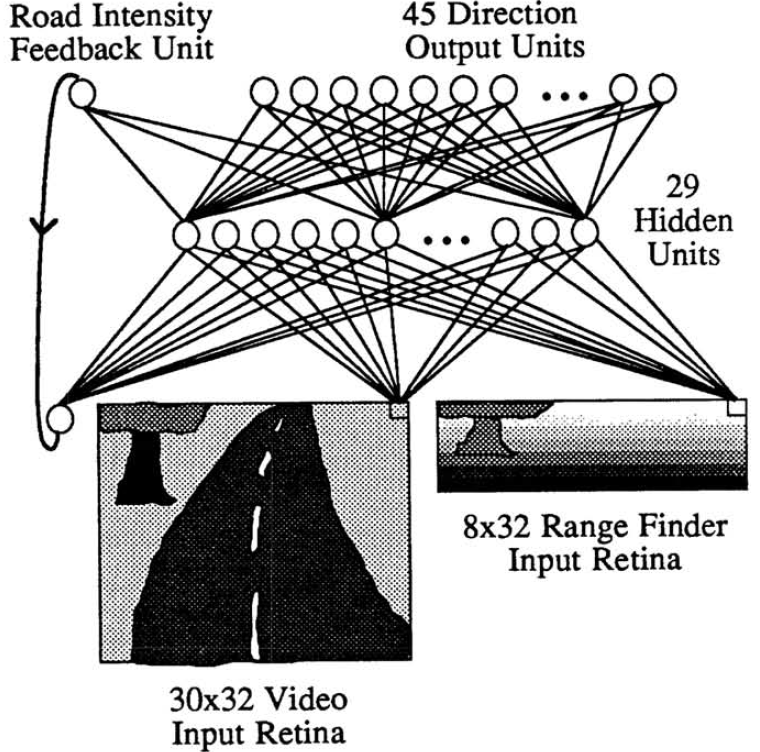
\includegraphics[scale=0.4]{src/pic/ALVINN.png}
%	\caption{The \nn called \alvinn and used as a behavior reflex based autonomous agent. \cite{pomerleau1989alvinn}}
%	\label{pic: ALVINN}
%\end{figure}

\section{Direct Perception}\label{sec: Direct Perception}

%In this paper we further analyze a suggested third group, called direct perception, which can traced to \cite{gibson2014ecological} in the late 80's, but was sharply criticized by researchers of the other two groups, i.e. in \cite{ullman1980against}.

The direct perception is the third group of approaches, which can be dated back to the 1954 and was initially mainly researched by James J. Gibson. \cite{gibson1954theory} The approach is based on analyzing a picture, not simply deducing a steering angle, or velocity change, like the behavior reflex approaches (cf. \Cref{sec: Behavior Reflex}), but also performing further computation without parsing it into a 3D world state model like the mediated perception approaches (cf. \Cref{sec: Mediated Perception}). \cite{chen2015deepdriving}\\
So it is a third paradigm, which can be interpreted as a hybrid of the two other paradigms. The approach tries to identify only the meaningful affordance indicators and make a decision based on those parameters. 

The CNN gets trained to make a reasonable assumption about the distance of other vehicles, their velocity and lane marks. These assumptions are further called affordance indicators.

We further consider a design based on \cite{chen2015deepdriving} and their way of training.

The original paper \cite{chen2015deepdriving} stated a total number of 13 indicators separated into two states to be sufficient for their design of a highway only autonomous agent. The states are: in line driving (following the lane) and on line driving (changing lanes). The values themselves can be categorized as: preceding car distances, distances to the lane markers and the steering angle. The indicators and their affiliation to the states can be seen in \Cref{lst: affordance indicators}.

\begin{figure}
\centering
\todoLine
\begin{lstlisting}[ basicstyle=\scriptsize]
always:
  1) angle: angle between the car's heading and the tangent of the road
i) "in lane system", when driving in the lane:
  2) toMarking LL: distance to the left lane marking of the left lane
  3) toMarking ML: distance to the left lane marking of the current lane
  4) toMarking MR: distance to the right lane marking of the current lane
  5) toMarking RR: distance to the right lane marking of the right lane
  6) dist LL: distance to the preceding car in the left lane
  7) dist MM: distance to the preceding car in the current lane
  8) dist RR: distance to the preceding car in the right lane
ii) "on marking system", when driving on the lane marking:
  9) toMarking L: distance to the left lane marking
  10) toMarking M: distance to the central lane marking
  11) toMarking R: distance to the right lane marking
  12) dist L: distance to the preceding car in the left lane
  13) dist R: distance to the preceding car in the right lane
\end{lstlisting}

\todoLine
\caption{The affordance indicators and their affiliation states}
\label{lst: affordance indicators}
\end{figure}

Based on the current state, all affordance indicators of the other state are not used, since the other state is defined to be inactive.\\
In order to identify the current state the host car is in, every state has their respective region, where they are active with an overlapping region for smooth transitioning.

Training is done by feeding the CNN with images of a current driving scenario as input and give estimated values to the mentioned affordance indicators active in the current state. Those values get forwarded to a controller dealing with the car. In the original approach the training was done via the \torcs game further explained in TODO %TODO: ref

The controller is setup to take the affordance values and compute a decision from it in an imperative way. For example the steering can be computed as 
	$$ steerCmd = C \cdot (angle-\frac{dist\_center}{road\_width})$$
where $dist\_center$ is the center of the current state (line we are on or middle of the lane), a coefficient $C$ suited for the current conditions, like weather or speed, and $angle\in [-\pi, \pi]$ as the affordance indicator.

Also using the controller to compute the accelerating and braking one can adjust the desired speed ($desired\_speed$) based on the affordance indicators. The $desired\_speed$ is set to the speed the agent wants to drive and can drop if a drastic steering motion is considered or accelerate to overtake a slower car.\\
In a one lane scenario with a  preceding car driving slower than the $desired\_speed$ there is no space to overtake. For that the controller has the velocity control car-following model:
	$$ v(t) = v_{max}(1-e^{-\frac{c\cdot dist(t)}{v_{max}} -d})$$ 
where $v_{max}$ is the maximal speed the agent is allowed to drive, $c$ and $d$ are coefficients specific to external conditions, like a wet lane or the cars potential of accelerating and braking, and $dist(t)$ is the distance to the preceding car. This distance is given through the trained CNN.

\begin{figure}
	\centering	
	\tikzset{->,very thick,>=stealth}
	\begin{subfigure}[b]{0.32\textwidth}
		\begin{tikzpicture}[scale=0.9] % top left picture
		\newcommand{\lineLength}{0.75}
		\newcommand{\lineSpace}{0.5}
		\newcommand{\startSpace}{0.25}
		
		\fill[green!50!black] (0,0) rectangle (5,5);		% background
		\fill[gray!50!black] (0.5,0) rectangle (4.5,5);     % pavement
		\fill[yellow!75!black] (0.55,0) rectangle (0.6,5);  % left yellow line
		\fill[yellow!75!black] (4.4,0) rectangle (4.45,5);  % right yellow line
		
		% left lane breaks		
		\fill[white] (1.84,\startSpace) rectangle (1.86,\lineLength+\startSpace);		
		\fill[white] (1.84,1*\lineLength + 1*\lineSpace + \startSpace) rectangle (1.86,2*\lineLength + 1*\lineSpace + \startSpace);
		\fill[white] (1.84,2*\lineLength + 2*\lineSpace + \startSpace) rectangle (1.86,3*\lineLength + 2*\lineSpace + \startSpace);
		\fill[white] (1.84,3*\lineLength + 3*\lineSpace + \startSpace) rectangle (1.86,4*\lineLength + 3*\lineSpace + \startSpace);
		
		% right line breaks
		\fill[white] (3.12,\startSpace) rectangle (3.14,\lineLength+\startSpace);		
		\fill[white] (3.12,1*\lineLength + 1*\lineSpace + \startSpace) rectangle (3.14,2*\lineLength + 1*\lineSpace + \startSpace);
		\fill[white] (3.12,2*\lineLength + 2*\lineSpace + \startSpace) rectangle (3.14,3*\lineLength + 2*\lineSpace + \startSpace);
		\fill[white] (3.12,3*\lineLength + 3*\lineSpace + \startSpace) rectangle (3.14,4*\lineLength + 3*\lineSpace + \startSpace);
		
		% cars
		\fill[red] (2.1,0.2) rectangle (2.1 + 0.8,0.2 + 1.5);	% agent		
		\fill[orange] (0.8,3.9) rectangle (0.8 + 0.8,3.9 + 1.1);	% left other car
		\fill[orange] (2.1,2.6) rectangle (2.1 + 0.8,2.6 + 1.5);	% middle other car
		\fill[orange] (3.4,3.2) rectangle (3.4 + 0.8,3.2 + 1.5);	% right other car
		\end{tikzpicture}
		\caption{slower car in the same lane}
		\label{fig: affordance indicators: in lane - lines}
	\end{subfigure}
	\begin{subfigure}[b]{0.32\textwidth}
		\begin{tikzpicture}[scale=0.9] % top middles picture
		\newcommand{\lineLength}{0.75}
		\newcommand{\lineSpace}{0.5}
		\newcommand{\startSpace}{0.25}
		
		\fill[green!50!black] (0,0) rectangle (5,5);		% background
		\fill[gray!50!black] (0.5,0) rectangle (4.5,5);     % pavement
		\fill[yellow!75!black] (0.55,0) rectangle (0.6,5);  % left yellow line
		\fill[yellow!75!black] (4.4,0) rectangle (4.45,5);  % right yellow line
		
		% left lane breaks		
		\fill[white] (1.84,\startSpace) rectangle (1.86,\lineLength+\startSpace);		
		\fill[white] (1.84,1*\lineLength + 1*\lineSpace + \startSpace) rectangle (1.86,2*\lineLength + 1*\lineSpace + \startSpace);
		\fill[white] (1.84,2*\lineLength + 2*\lineSpace + \startSpace) rectangle (1.86,3*\lineLength + 2*\lineSpace + \startSpace);
		\fill[white] (1.84,3*\lineLength + 3*\lineSpace + \startSpace) rectangle (1.86,4*\lineLength + 3*\lineSpace + \startSpace);
		
		% right line breaks
		\fill[white] (3.12,\startSpace) rectangle (3.14,\lineLength+\startSpace);		
		\fill[white] (3.12,1*\lineLength + 1*\lineSpace + \startSpace) rectangle (3.14,2*\lineLength + 1*\lineSpace + \startSpace);
		\fill[white] (3.12,2*\lineLength + 2*\lineSpace + \startSpace) rectangle (3.14,3*\lineLength + 2*\lineSpace + \startSpace);
		\fill[white] (3.12,3*\lineLength + 3*\lineSpace + \startSpace) rectangle (3.14,4*\lineLength + 3*\lineSpace + \startSpace);
		
		% cars
		\fill[red] (2.1,0.2) rectangle (2.1 + 0.8,0.2 + 1.5);
		\fill[orange] (0.8,3.9) rectangle (0.8 + 0.8,3.9 + 1.1);	% left other car
		\fill[orange] (2.1,2.6) rectangle (2.1 + 0.8,2.6 + 1.5);	% middle other car
		\fill[orange] (3.4,3.2) rectangle (3.4 + 0.8,3.2 + 1.5);	% right other car
		\end{tikzpicture}
		\caption{equal fast car in same lane}
		\label{fig: affordance indicators: in lane - cars}
	\end{subfigure}
	\begin{subfigure}[b]{0.32\textwidth}
		\begin{tikzpicture}[scale=0.9] % top left picture
		\newcommand{\lineLength}{0.75}
		\newcommand{\lineSpace}{0.5}
		\newcommand{\startSpace}{0.25}
		
		\fill[green!50!black] (0,0) rectangle (5,5);		% background
		
%		\draw [-,gray!50!black,thick,domain=0:60] plot ({2.5*cos(\x)-1.25}, {2.5*sin(\x)});
%		\draw [-,gray!50!black,thick,domain=16:50] plot ({6.5*cos(\x)-1.25}, {6.5*sin(\x)});
%		\fill[gray!50!black] (0.5,0) rectangle (4.5,5);     % pavement
		
%		\fill[yellow!75!black] (0.55,0) rectangle (0.6,5);  % left yellow line
%		\fill[yellow!75!black] (4.4,0) rectangle (4.45,5);  % right yellow line
		
		% left lane breaks		
%		\fill[white] (1.84,\startSpace) rectangle (1.86,\lineLength+\startSpace);		
%		\fill[white] (1.84,1*\lineLength + 1*\lineSpace + \startSpace) rectangle (1.86,2*\lineLength + 1*\lineSpace + \startSpace);
%		\fill[white] (1.84,2*\lineLength + 2*\lineSpace + \startSpace) rectangle (1.86,3*\lineLength + 2*\lineSpace + \startSpace);
%		\fill[white] (1.84,3*\lineLength + 3*\lineSpace + \startSpace) rectangle (1.86,4*\lineLength + 3*\lineSpace + \startSpace);
		
		% right line breaks
%		\fill[white] (3.12,\startSpace) rectangle (3.14,\lineLength+\startSpace);		
%		\fill[white] (3.12,1*\lineLength + 1*\lineSpace + \startSpace) rectangle (3.14,2*\lineLength + 1*\lineSpace + \startSpace);
%		\fill[white] (3.12,2*\lineLength + 2*\lineSpace + \startSpace) rectangle (3.14,3*\lineLength + 2*\lineSpace + \startSpace);
%		\fill[white] (3.12,3*\lineLength + 3*\lineSpace + \startSpace) rectangle (3.14,4*\lineLength + 3*\lineSpace + \startSpace);
		
		% cars
%		\fill[red] (2.1,0.2) rectangle (2.1 + 0.8,0.2 + 1.5);
		
		%		\node [trapezium, minimum width = 3.6cm, trapezium angle=25,rotate = 180, opacity = 0.4, color = gray!50!white, fill] at (2.5,2) (test) {};
		%		\fill[gray!50!white, opacity = 0.4] (0.5,2.378) rectangle (4.5,5);
		\end{tikzpicture}
		\caption{}
		\label{fig: affordance indicators: angle}
	\end{subfigure}
	
	\begin{subfigure}[b]{0.32\textwidth}
		\begin{tikzpicture}[scale=0.9] % bottom left picture
		\newcommand{\lineLength}{0.75}
		\newcommand{\lineSpace}{0.5}
		\newcommand{\startSpace}{0.25}
		
		\fill[green!50!black] (0,0) rectangle (5,5);		% background
		\fill[gray!50!black] (0.5,0) rectangle (4.5,5);     % pavement
		\fill[yellow!75!black] (0.55,0) rectangle (0.6,5);  % left yellow line
		\fill[yellow!75!black] (4.4,0) rectangle (4.45,5);  % right yellow line
		
		% left lane breaks		
		\fill[white] (1.84,\startSpace) rectangle (1.86,\lineLength+\startSpace);		
		\fill[white] (1.84,1*\lineLength + 1*\lineSpace + \startSpace) rectangle (1.86,2*\lineLength + 1*\lineSpace + \startSpace);
		\fill[white] (1.84,2*\lineLength + 2*\lineSpace + \startSpace) rectangle (1.86,3*\lineLength + 2*\lineSpace + \startSpace);
		\fill[white] (1.84,3*\lineLength + 3*\lineSpace + \startSpace) rectangle (1.86,4*\lineLength + 3*\lineSpace + \startSpace);
		
		% right line breaks
		\fill[white] (3.12,\startSpace) rectangle (3.14,\lineLength+\startSpace);		
		\fill[white] (3.12,1*\lineLength + 1*\lineSpace + \startSpace) rectangle (3.14,2*\lineLength + 1*\lineSpace + \startSpace);
		\fill[white] (3.12,2*\lineLength + 2*\lineSpace + \startSpace) rectangle (3.14,3*\lineLength + 2*\lineSpace + \startSpace);
		\fill[white] (3.12,3*\lineLength + 3*\lineSpace + \startSpace) rectangle (3.14,4*\lineLength + 3*\lineSpace + \startSpace);
		
		% cars
		\fill[red] (1.5,0.2) rectangle (1.5 + 0.8,0.2 + 1.5);
		\fill[orange] (0.8,3.9) rectangle (0.8 + 0.8,3.9 + 1.1);	% left other car
		\fill[orange] (2.1,2.6) rectangle (2.1 + 0.8,2.6 + 1.5);	% middle other car
		\fill[gray!50!white] (3.4,3.2) rectangle (3.4 + 0.8,3.2 + 1.5);	% right other car
		%		\node [trapezium, minimum width = 3.6cm, trapezium angle=25,rotate = 180, opacity = 0.4, color = gray!50!white, fill] at (2.5,2) (test) {};
		%		\fill[gray!50!white, opacity = 0.4] (0.5,2.378) rectangle (4.5,5);
		\end{tikzpicture}
		\caption{free lane}
		\label{fig: affordance indicators: on lane - lines}
	\end{subfigure}
	\begin{subfigure}[b]{0.32\textwidth}
		\begin{tikzpicture}[scale=0.9] % bottom middle picture
		\newcommand{\lineLength}{0.75}
		\newcommand{\lineSpace}{0.5}
		\newcommand{\startSpace}{0.25}
		
		\fill[green!50!black] (0,0) rectangle (5,5);		% background
		\fill[gray!50!black] (0.5,0) rectangle (4.5,5);     % pavement
		\fill[yellow!75!black] (0.55,0) rectangle (0.6,5);  % left yellow line
		\fill[yellow!75!black] (4.4,0) rectangle (4.45,5);  % right yellow line
		
		% left lane breaks		
		\fill[white] (1.84,\startSpace) rectangle (1.86,\lineLength+\startSpace);		
		\fill[white] (1.84,1*\lineLength + 1*\lineSpace + \startSpace) rectangle (1.86,2*\lineLength + 1*\lineSpace + \startSpace);
		\fill[white] (1.84,2*\lineLength + 2*\lineSpace + \startSpace) rectangle (1.86,3*\lineLength + 2*\lineSpace + \startSpace);
		\fill[white] (1.84,3*\lineLength + 3*\lineSpace + \startSpace) rectangle (1.86,4*\lineLength + 3*\lineSpace + \startSpace);
		
		% right line breaks
		\fill[white] (3.12,\startSpace) rectangle (3.14,\lineLength+\startSpace);		
		\fill[white] (3.12,1*\lineLength + 1*\lineSpace + \startSpace) rectangle (3.14,2*\lineLength + 1*\lineSpace + \startSpace);
		\fill[white] (3.12,2*\lineLength + 2*\lineSpace + \startSpace) rectangle (3.14,3*\lineLength + 2*\lineSpace + \startSpace);
		\fill[white] (3.12,3*\lineLength + 3*\lineSpace + \startSpace) rectangle (3.14,4*\lineLength + 3*\lineSpace + \startSpace);
		
		% cars
		\fill[red] (1.5,0.2) rectangle (1.5 + 0.8,0.2 + 1.5);
		\fill[orange] (0.8,3.9) rectangle (0.8 + 0.8,3.9 + 1.1);	% left other car
		\fill[orange] (2.1,2.6) rectangle (2.1 + 0.8,2.6 + 1.5);	% middle other car
		\fill[gray!50!white] (3.4,3.2) rectangle (3.4 + 0.8,3.2 + 1.5);	% right other car
		\end{tikzpicture}
		\caption{slower car in the same lane}
		\label{fig: affordance indicators: on lane - cars}
	\end{subfigure}
	\begin{subfigure}[b]{0.32\textwidth}
		\begin{tikzpicture}[scale=0.9] % bottom right picture
		\newcommand{\lineLength}{0.75}
		\newcommand{\lineSpace}{0.5}
		\newcommand{\startSpace}{0.25}
		
		\fill[green!50!black] (0,0) rectangle (5,5);		% background
		\fill[gray!50!black] (0.5,0) rectangle (4.5,5);     % pavement
		\fill[yellow!75!black] (0.55,0) rectangle (0.6,5);  % left yellow line
		\fill[yellow!75!black] (4.4,0) rectangle (4.45,5);  % right yellow line
		
		
		% overlapping areas
		\fill[black] (1.4,0.5) rectangle (1.4+0.15,0.5 + 4);
		\fill[gray!75!black] (1.55,0.5) rectangle (1.55 + 0.6,0.5 + 4);
		\fill[black] (2.15,0.5) rectangle (2.15+0.15,0.5 + 4);
		
		\fill[black] (1.4 +1.25,0.5) rectangle (1.4+0.15 +1.25,0.5 + 4);
		\fill[gray!75!black] (1.55 + 1.25 ,0.5) rectangle (1.55 + 0.6 +1.25,0.5 + 4);
		\fill[black] (2.15 +1.25,0.5) rectangle (2.15+0.15 +1.25,0.5 + 4);
		
		% left lane breaks		
		\fill[white] (1.84,\startSpace) rectangle (1.86,\lineLength+\startSpace);		
		\fill[white] (1.84,1*\lineLength + 1*\lineSpace + \startSpace) rectangle (1.86,2*\lineLength + 1*\lineSpace + \startSpace);
		\fill[white] (1.84,2*\lineLength + 2*\lineSpace + \startSpace) rectangle (1.86,3*\lineLength + 2*\lineSpace + \startSpace);
		\fill[white] (1.84,3*\lineLength + 3*\lineSpace + \startSpace) rectangle (1.86,4*\lineLength + 3*\lineSpace + \startSpace);
		
		% right line breaks
		\fill[white] (3.12,\startSpace) rectangle (3.14,\lineLength+\startSpace);		
		\fill[white] (3.12,1*\lineLength + 1*\lineSpace + \startSpace) rectangle (3.14,2*\lineLength + 1*\lineSpace + \startSpace);
		\fill[white] (3.12,2*\lineLength + 2*\lineSpace + \startSpace) rectangle (3.14,3*\lineLength + 2*\lineSpace + \startSpace);
		\fill[white] (3.12,3*\lineLength + 3*\lineSpace + \startSpace) rectangle (3.14,4*\lineLength + 3*\lineSpace + \startSpace);
		\end{tikzpicture}
		\caption{equal fast car in same lane}
		\label{fig: affordance indicators: overlapping areas}
	\end{subfigure}
	
	\caption{The 3 scenarios causing problems with behavior reflex approaches. The red block is the agent, the orange block the other car, the white arrows indicate the velocity and the green arrows the logically deduced behaviors.}
	\label{fig: behavior sketches}
\end{figure}

%\todo{\begin{enumerate}
%\item show graphic of how controller computes
%\end{enumerate}}



\chapter{Comparison: \cnnarch \& \caffe}\label{chapter: Comparison}

In this chapter we want to compare the \alexnet (c.f. \Cref{sec: AlexNet}) implemented using \cnnarch and \caffe. This net is used in the direct perception approach (c.f. \Cref{sec: Direct Perception}) and therefore crucial for its performance. For both we take an in depth look at the predefined architecture by their respective language. We do that, since both implementations are done by language experts and build to be as efficient and precise in the language as possible.

Further, we state the currently most used methods to train an autonomous driving agent. Those training methods are also used for the approaches in \Cref{chapter: Deep Learning Approaches}. The important properties required are stated.


\section{Implementation} \label{sec: Implementation}

\subsection{\caffe} \label{subsec: Caffe Implementation}
The implementation of the \alexnet using \caffe is given partly in \Cref{lst: Caffe AlexNet}. The whole net has a total number of 284 lines. Obviously the code was written very verbosely. Every layer has to be explicitly specified, even if they have a very similar structure to a previous layer.

%\newpage  %TODO restructure
For example comparing the pooling layer ``pool1'' from line 51 to 61 and the pooling layer ``pool2'' from line 99 to 109 in \Cref{lst: pool1 and pool2}:
\begin{figure}[H]
	\centering
	\begin{subfigure}[b]{0.45\textwidth}
		\hspace*{2cm}\vdots
		\lstinputlisting[numbers=left, firstnumber = 51, basicstyle=\scriptsize,firstline=51, lastline=61]{src/listing/alexnet.prototxt}
		\hspace*{2cm}\vdots
		\caption{``pool1''}
		\label{lst: pool1}
	\end{subfigure}
	\begin{subfigure}[b]{0.45\textwidth}
		\hspace*{2cm}\vdots
		\lstinputlisting[numbers=left, firstnumber = 99, basicstyle=\scriptsize,firstline=99, lastline=109]{src/listing/alexnet.prototxt}
		\hspace*{2cm}\vdots
		\caption{``pool2''}
		\label{lst: pool2}
	\end{subfigure}
	\caption{}
	\label{lst: pool1 and pool2}
\end{figure}
The lines first 3 and last 6 lines are completely similar. The other 2 lines are just different regarding the name of the incoming and outgoing connections. Creating a huge and deep net would lead to an enormously large description file. 

\subsection{\cnnarch} \label{subsec: CNNArch Implementation}

The implementation of the \alexnet using \cnnarch can be seen in \Cref{lst: CNNArchLang AlexNet}. The complete script has 43 lines and defines the same net construction as the 284 line definition in \caffe. This shows the efficient language design used in the creation of \cnnarch (c.f. \Cref{sec: CNNArch}). \\
The two pooling operations of \Cref{lst: pool1 and pool2} can be located in line 32 using the Python like syntax of definition and the sequential connection \texttt{->} (c.f. \Cref{item: sequential connection}).

Using those techniques \cnnarch is able to write even complex \nn using a few lines of code. This and the syntax itself create an easy to read program.

\subsection{Comparison}
Due to complications regarding the \cnnarch-inclusion in an existing program infrastructure, as well as \caffe, currently having issues with their build-script there is no possibility to directly compare times taken for training the \nn. \\
Nevertheless based on the usage of \mxnet, by \cnnarch (c.f. \Cref{subsec: CNNArch Implementation} and \Cref{chapter: conclusion}), it is suspected to be much faster than the \caffe approach.\\
About the effectiveness and other performance indicators, such as error rate, there can not be any profound reasoning without an actual implementation and testing.

\section{Training}

In order to train a CNN, independent of the underlying approach (c.f. \Cref{chapter: DLL}), one has to obtain a huge database of input images and the labels, i.e. actions or values the CNN should have computed. For autonomous driving the training has to be rigorous. Otherwise the car driven by the agent will take damage by just slight changes of the circumstances.\\
Also different scenarios have to be trained. Only training the driving on a road without other cars and simply following the lane is a very disparate task compared to overtaking a slower car.\\
For that, the following sources of such databases are currently state-of-the-art.

\subsection{KITTI Dataset} \label{subsec: KITTI}

The \kitti dataset is a 6 hour recoding by the Karlsruhe Institute of Technology. They mounted various cameras and laser scanners on a VW Passat and drove around the german city Karlsruhe.\\
During those hours they collected a total amount of 180 GB of data. This data includes images, in different channels from the drivers point of view, sensor data of distances, steering angle, acceleration/braking, current speed, GPS coordinates, and others. \\
While other test sets are often developed using a very specific setup for a corresponding approach, the \kitti dataset has such a high variety of data captured, resulting in many appearances in other scientific papers. It has become one of the default datasets to compare different approaches on. \cite{KITTI}

\subsection{TORCS} \label{subsec: TORCS}

A game called \textbf{T}he \textbf{O}pen \textbf{R}acing \textbf{C}ar \textbf{S}imulator or short \torcs is a racing game specially designed for artificial intelligence research. It is designed to be modular in order to retrieve every kind of data one needs for their approach. It also offers a documented API, to create for example a driving agent. 

The possibility to collect any kind of data is what makes this game so popular in current research. The advantage over the \kitti dataset is that, if one needs a very specific value not included within the \kitti dataset, the approach can not be trained with it. Neglecting, whether such a value is meaningful in terms of the ability to collect it during real driving, there would be an other specialized set collecting only the data this specific approach needs. But this specialized set may lack a value, which is required in order to compare it with an another approach. So there is no common training set, on which a comparison could base.

% and maybe not collecting the data one needs to compare it to an other approach.

The disadvantage of the training via \torcs compared to training via \kitti is, that \torcs only uses artificial images, other artificial agents, and is completely exempt from any kind of data noise, like rain disturbing sensor data or sunlight blending the camera. Also other cars behave different in a game than in real life. The \kitti includes some of those problems. To which extend is arguable. \cite{wymann2000torcs}



\chapter{Evaluation of Direct Perception}

In this chapter we take a look back at the direct perception approach and evaluate its performance. For that we compare the, via \torcs (c.f. \Cref{subsec: TORCS}), trained version to a behavior reflex approach (c.f. \Cref{sec: Behavior Reflex}). In addition to that there is also a comparison of the direct perception approach, trained via \kitti (c.f. \Cref{subsec: KITTI}), to a mediated perception approach stated in \cite{geiger20143d}.\\
We base the comparison on the running examples in \cite{DeepDriving}, which were written using \caffe.\\
Finally we take a look at possible scenarios causing problems which may emerge. 

The directed perception as stated in \cite{chen2015deepdriving} and discussed in \Cref{sec: Direct Perception} is designed to handle highway driving tasks, such as driving in a lane, overtaking slower cars, detecting the lane configuration and breaking to avoid a collision.


\begin{wrapfigure}[15]{r}{4cm}
	\vspace*{-1em}
	\begin{tikzpicture}[scale=0.9] % middle picture
	\newcommand{\lineLength}{0.75}
	\newcommand{\lineSpace}{0.5}
	\newcommand{\startSpace}{0.25}
	
	\fill[green!50!black] (0,0) rectangle (5,5);		% background
	\fill[gray!50!black] (0.5,0) rectangle (4.5,5);     % pavement
	\fill[yellow!75!black] (0.55,0) rectangle (0.6,5);  % left yellow line
	\fill[yellow!75!black] (4.4,0) rectangle (4.45,5);  % right yellow line
	
	% left lane breaks		
	\fill[white] (1.84,\startSpace) rectangle (1.86,\lineLength+\startSpace);		
	\fill[white] (1.84,1*\lineLength + 1*\lineSpace + \startSpace) rectangle (1.86,2*\lineLength + 1*\lineSpace + \startSpace);
	\fill[white] (1.84,2*\lineLength + 2*\lineSpace + \startSpace) rectangle (1.86,3*\lineLength + 2*\lineSpace + \startSpace);
	\fill[white] (1.84,3*\lineLength + 3*\lineSpace + \startSpace) rectangle (1.86,4*\lineLength + 3*\lineSpace + \startSpace);
	
	% right line breaks
	\fill[white] (3.12,\startSpace) rectangle (3.14,\lineLength+\startSpace);		
	\fill[white] (3.12,1*\lineLength + 1*\lineSpace + \startSpace) rectangle (3.14,2*\lineLength + 1*\lineSpace + \startSpace);
	\fill[white] (3.12,2*\lineLength + 2*\lineSpace + \startSpace) rectangle (3.14,3*\lineLength + 2*\lineSpace + \startSpace);
	\fill[white] (3.12,3*\lineLength + 3*\lineSpace + \startSpace) rectangle (3.14,4*\lineLength + 3*\lineSpace + \startSpace);
	
	% cars
	\fill[red] (2.1,0.2) rectangle (2.1 + 0.8,0.2 + 1.5);	% agent
	\draw[->,very thick,  color = white] (2.5,0.4) -- (2.5,1.2);
	\draw[->,very thick,  color = red!75!black] (2,1.8) -- (1.3,2.5) -- (1.3,3);
	
	
	\fill[orange] (2.1,3.2) rectangle (2.1 + 0.8,3.2 + 1.5);	% other car
	\draw[->,very thick,  color = white] (2.5,3.4) -- (2.5,4);
	
	\fill[orange] (0.8,0) rectangle (0.8 + 0.8,0 + 1.1);	% other car
	\draw[->,very thick,  color = white] (1.2,0) -- (1.2,1);
	\end{tikzpicture}
	\caption{A scenario that has to be considered to create a full autonomous driving agent}
	\label{fig: behavior sketche complex scenario}
\end{wrapfigure}

The behavior reflex approach was able to follow empty lanes perfectly, but was completely unable to have a acceptable behavior considering other cars. Neither a sufficient speed regulation nor the task of staying in lane was observable. The agent left the track various times and had multiple collisions.\\
On the other hand the direct perception approach manages to change lanes smoothly to avoid collisions and stay in lane. Due to the speed regulation in the controller, stated in \Cref{sec: Direct Perception}, the agent is able to perform an emergency brake if necessary. So considering those scenarios the direct perception outperforms the behavior reflex approach.

In order to compare with the state-of-the-art mediated perception approach, the training is done using the \kitti dataset and also combine two CNNs for near and far perception, both using the direct perception approach. It shows that the direct perception approach is able to perform roughly as good, even though they restrict themselves to the cars closest to the host car. So the direct perception is sufficient for real world examples as well. \cite{DeepDriving} \cite{chen2015deepdriving}

Despite the two mentioned comparisons there are still others that need further investigation. Considering more complex tasks, which mediated perception approaches are able to handle, the direct perception needs to prove itself.
Considering classification tasks like road signs, pedestrians detection or traffic light detection including its current light showing still have to be done in order to create a sufficient agent for real-life cars. 
Also more complex scenarios like busy intersections have to be solved. Also scenarios as sketched in \Cref{fig: behavior sketche complex scenario}, where the overtaking can not take place since a car left and possibly a bit behind of the host is even faster.
A number of those scenarios can be managed by a sophisticated controller, but this would again take more time and provides less flexibility.

So concluding the direct perception definitely is state-of-the-art and has the potential to found the base of a sophisticated autonomous driving agent, if considered as a predictor of distances they call affordance indicators. But whether or not the direct perception can handle a complete real-life scenario is still up to prove.


%\chapter{Code Listings}\label{ch:listings}
%% use language 'myLng' for the next listings (until another language is set)
%% include listing 'listings/AdverseReactionApp.aj' with label and caption
%% note: big listings sometimes need to overwrite the float value that has been
%% already set in the general listings setup (see paper.tex)

This chapter contains the beautiful listing \ref{lst:system}. 
Lorem ipsum dolor sit amet, consetetur sadipscing elitr, sed diam nonumy 
eirmod tempor invidunt ut labore et dolore magna aliquyam erat, sed diam 
voluptua. At vero eos et accusam et justo duo dolores et ea rebum. Stet 
clita kasd gubergren, no sea takimata sanctus est Lorem ipsum dolor sit 
amet. Lorem ipsum dolor sit amet, consetetur sadipscing elitr, sed diam 
nonumy eirmod tempor invidunt ut labore et dolore magna aliquyam erat, 
sed diam voluptua. At vero eos et accusam et justo duo dolores et ea 
rebum. Stet clita kasd gubergren, no sea takimata sanctus est Lorem 
ipsum dolor sit amet. 




\begin{figure}[hbt]
\lstset{language=MontiArc}
\lstinputlisting[
label=lst:system,
caption=Code listing with user defined syntax highlighting (MontiArc).] {src/listings/AdverseReactionApp.aj}
\end{figure}

\cleardoublepage


\chapter{Conclusion}

Conclusion of differences and similarities between the frameworks\\

\begin{tabular}{l |c |c |c |c }
	Property 						& \cnnarch 		& \caffe 		& \caffetwo 		& \mxnet \\ \hline
					\multicolumn{5}{c}{General Information}\\\hline
	is full framework  				& \xmark		& \cmark		& \cmark			& \cmark \\
	SLI usage						& -- 			& \xmark$^1$ 	& \xmark$^1$ 		& \cmark \\
	mult. computers 				& -- 			& \cmark		& \cmark			& \cmark \\	
	\hline
					\multicolumn{5}{c}{Nets Supported}\\ \hline
	typical CNNs					& \cmark		& \cmark		& \cmark			& \cmark \\
	arbitrary CNNs					& \xmark		& \cmark		& \cmark			& \cmark \\
	Recurrent NNs					& \xmark		& \cmark		& \cmark			& \cmark \\
	\hline
					\multicolumn{5}{c}{Constructs}\\ \hline
	predefined NNs					& \cmark		& \cmark		& \cmark			& \cmark \\
	pretrained NNs  				& \xmark		& \cmark		& \xmark$^2$		& \cmark \\
	simple arbitrary net creation	& \cmark		& \xmark 		& \xmark			& \cmark \\	
	predefined functions 		  	& \cmark		& \cmark		& \cmark			& \cmark \\
	simple function creation 	  	& \cmark 		& \xmark		& \xmark$^2$		& \cmark \\
	low-level operations			& \xmark		& \xmark		& \xmark			& \cmark \\ %check
	\hline
					\multicolumn{5}{c}{Language bindings}\\ \hline
	C++								& \xmark		& \cmark		& \cmark			& \cmark \\
	Python							& \cmark		& \xmark$^3$	& \cmark			& \cmark \\
	MatLab							& ? 			& \cmark		& \xmark			& \cmark \\ 
	Others							& ?				& ?				& ?					& R, Go, Julia, Perl\\
									&				&				&					& JavaScript, Scala \\ 
%	\hline
%					\multicolumn{5}{c}{Usage}\\ \hline
%					understandability & & & & \\
%					handling & & & & \\
\end{tabular}

\begin{itemize}
	\item[$^1$] depending on CUDA version/installation
	\item[$^2$] not clearly stated, but also not denied
	\item[$^3$] added lately
\end{itemize}

Possible Criteria%SEE: 4.4.1 in CNNArchLang
\begin{itemize}
	\item generality
	\item expressiveness
	\item modularity
	\item is Framework?
	\item Installation 
	\item Error Handling
	\item for equal task?
	\item low-level computations
\end{itemize}
Also a general conclusion based on results and \cite{grzywaczewski2017training}

\chapter{Appendix}
\vspace*{-4em}
\begin{figure}[H]
\begin{minipage}[t]{0.33\textwidth}
	\lstinputlisting[numbers=left, basicstyle=\scriptsize,firstline=1, lastline=51]{src/listing/alexnet.prototxt}
\end{minipage}
\begin{minipage}[t]{0.33\textwidth}
	\lstinputlisting[numbers=left, firstnumber = 51, basicstyle=\scriptsize,firstline=51, lastline=101]{src/listing/alexnet.prototxt}
\end{minipage}
\begin{minipage}[t]{0.33\textwidth}
	\lstinputlisting[numbers=left, firstnumber = 101, basicstyle=\scriptsize,firstline=101, lastline=139]{src/listing/alexnet.prototxt}
	\hspace*{2cm}\vdots
\end{minipage}

\caption{The \caffe implementation of the \alexnet. This is only the first 169 lines. The whole net has a size of 284 lines of code. The main reason of this is the highly verbose Protocol Buffer prototxt style. Further explanation in \Cref{sec: Caffe}. \cite{CaffeAlexNetGithub}}
\label{lst: Caffe AlexNet}
\end{figure}

\begin{figure}
	%	\centering
	\todoLine
	\hspace*{-0.5cm}
	\lstinputlisting[numbers = left, basicstyle=\scriptsize]{src/listing/alexnet.txt}
	\todoLine
	\caption{The \alexnet implemented in \cnnarch. This is the whole program to describe the whole net. Further explanation in \Cref{sec: CNNArch}. \cite{CNNArch}}
	\label{lst: CNNArchLang AlexNet}
\end{figure}

\bibliographystyle{alpha}
\addcontentsline{toc}{chapter}{Literaturverzeichnis}
\bibliography{src/bib/Literatur}

% Begin Anhang
%\appendix
%\chapter{z.\,B. Programmdokumentation}

\cleardoublepage


\end{document}
